% !TeX program = xelatex
\documentclass[11pt,a4paper,oneside]{report}

% ---------- Page and fonts ----------
\usepackage[top=16mm,bottom=18mm,left=18mm,right=18mm,includefoot]{geometry}
\usepackage{fontspec}
\usepackage{xeCJK}
\setmainfont{Noto Sans}
\setsansfont{Noto Sans}
\setmonofont{Noto Sans Mono}
\setCJKmainfont{Noto Sans CJK TC}[BoldFont=Noto Sans CJK TC Bold]
\setCJKsansfont{Noto Sans CJK TC}[BoldFont=Noto Sans CJK TC Bold]
\setCJKmonofont{Noto Sans Mono CJK TC}
\renewcommand{\familydefault}{\sfdefault}

% ---------- Core packages ----------
\usepackage{amsmath,amssymb,mathtools}
\usepackage[table]{xcolor}
\usepackage{graphicx}
\usepackage{booktabs,tabularx,array,multirow,longtable}
\usepackage{enumitem}
\usepackage{titlesec}
\usepackage{fancyhdr}
\usepackage{tcolorbox}
\tcbuselibrary{breakable,skins,raster,theorems}
\usepackage{tikz}
\usetikzlibrary{arrows.meta,positioning,calc,fit,shapes.geometric,shadows.blur,matrix,backgrounds,decorations.pathreplacing}
\usepackage{pgfplots}
\pgfplotsset{compat=1.18}
\usepackage{hyperref}
\usepackage{bookmark}
\usepackage{microtype}
\usepackage{setspace}
\usepackage{ragged2e}
\usepackage{lastpage}
\usepackage{etoolbox}

% ---------- Color system ----------
\definecolor{Ink}{HTML}{172033}
\definecolor{Muted}{HTML}{5E6B7A}
\definecolor{Paper}{HTML}{F7F9FC}
\definecolor{Line}{HTML}{D8E1EC}
\definecolor{Teal}{HTML}{0A8F8D}
\definecolor{TealSoft}{HTML}{E7F7F6}
\definecolor{Blue}{HTML}{2F6FED}
\definecolor{BlueSoft}{HTML}{EAF0FF}
\definecolor{Orange}{HTML}{F28C28}
\definecolor{OrangeSoft}{HTML}{FFF2E2}
\definecolor{Purple}{HTML}{7756C8}
\definecolor{PurpleSoft}{HTML}{F1ECFF}
\definecolor{Pink}{HTML}{D64B7F}
\definecolor{PinkSoft}{HTML}{FCEAF1}
\definecolor{Green}{HTML}{2E9D63}
\definecolor{GreenSoft}{HTML}{EAF7F0}
\definecolor{Red}{HTML}{C94747}
\definecolor{RedSoft}{HTML}{FCECEC}
\definecolor{Yellow}{HTML}{E5B700}
\definecolor{Court}{HTML}{E8A85B}
\definecolor{CourtDark}{HTML}{B86E2D}

% ---------- Global typography ----------
\setlength{\parindent}{0pt}
\setlength{\parskip}{0.55em}
\setstretch{1.13}
\renewcommand{\arraystretch}{1.25}
\setlist[itemize]{leftmargin=1.5em,itemsep=0.3em,topsep=0.3em}
\setlist[enumerate]{leftmargin=1.65em,itemsep=0.35em,topsep=0.3em}
\newcolumntype{Y}{>{\RaggedRight\arraybackslash}X}
\newcolumntype{C}[1]{>{\Centering\arraybackslash}m{#1}}
\newcolumntype{R}[1]{>{\RaggedLeft\arraybackslash}m{#1}}

% ---------- Heading styles ----------
\titleformat{\chapter}[display]
  {\bfseries\color{Ink}}
  {\large\color{Muted}第 \thechapter 章}
  {5pt}
  {\Huge}
  [\vspace{4pt}\color{Line}\titlerule]
\titlespacing*{\chapter}{0pt}{-12pt}{20pt}
\titleformat{\section}{\Large\bfseries\color{Ink}}{}{0pt}{}
\titleformat{\subsection}{\large\bfseries\color{Blue}}{}{0pt}{}
\titleformat{\subsubsection}{\normalsize\bfseries\color{Purple}}{}{0pt}{}
\titlespacing*{\section}{0pt}{1.3em}{0.45em}
\titlespacing*{\subsection}{0pt}{1.05em}{0.3em}
\titlespacing*{\subsubsection}{0pt}{0.85em}{0.2em}

% ---------- Footer ----------
\pagestyle{fancy}
\fancyhf{}
\fancyfoot[C]{\small\color{Muted}\thepage}
\renewcommand{\headrulewidth}{0pt}
\renewcommand{\footrulewidth}{0pt}
\fancypagestyle{plain}{%
  \fancyhf{}
  \fancyfoot[C]{\small\color{Muted}\thepage}
  \renewcommand{\headrulewidth}{0pt}
  \renewcommand{\footrulewidth}{0pt}
}
\renewcommand{\bibname}{參考資料}

% ---------- Hyperlinks ----------
\hypersetup{
  colorlinks=true,
  linkcolor=Blue,
  urlcolor=Teal,
  citecolor=Purple,
  pdfauthor={},
  pdftitle={Python「黑客松」實戰分析籃球運動數據}
}

% ---------- Reusable boxes ----------
\newtcolorbox{heroBox}[1][]{
  enhanced,breakable,colback=TealSoft,colframe=Teal,
  boxrule=0.8pt,arc=4pt,left=10pt,right=10pt,top=8pt,bottom=8pt,
  borderline west={4pt}{0pt}{Teal},#1
}
\newtcolorbox{plainBox}[1][]{
  enhanced,breakable,colback=white,colframe=Line,
  boxrule=0.7pt,arc=4pt,left=9pt,right=9pt,top=7pt,bottom=7pt,#1
}
\newtcolorbox{conceptBox}[1][]{
  enhanced,breakable,colback=BlueSoft,colframe=Blue,
  boxrule=0.7pt,arc=4pt,title={\bfseries 概念導入},
  coltitle=white,colbacktitle=Blue,#1
}
\newtcolorbox{historyBox}[1][]{
  enhanced,breakable,colback=OrangeSoft,colframe=Orange,
  boxrule=0.7pt,arc=4pt,title={\bfseries 技術發展脈絡},
  coltitle=white,colbacktitle=Orange,#1
}
\newtcolorbox{toolBox}[1][]{
  enhanced,breakable,colback=PurpleSoft,colframe=Purple,
  boxrule=0.7pt,arc=4pt,title={\bfseries 常見工具與框架},
  coltitle=white,colbacktitle=Purple,#1
}
\newtcolorbox{riskBox}[1][]{
  enhanced,breakable,colback=RedSoft,colframe=Red,
  boxrule=0.7pt,arc=4pt,title={\bfseries 常見誤解與失敗模式},
  coltitle=white,colbacktitle=Red,#1
}
\newtcolorbox{takeawayBox}[1][]{
  enhanced,breakable,colback=GreenSoft,colframe=Green,
  boxrule=0.7pt,arc=4pt,title={\bfseries 本節重點},
  coltitle=white,colbacktitle=Green,#1
}
\newtcolorbox{termBox}[2][]{
  enhanced,breakable,colback=white,colframe=Line,
  boxrule=0.6pt,arc=3pt,left=8pt,right=8pt,top=6pt,bottom=6pt,
  title={\bfseries\color{Ink}#2},colbacktitle=Paper,coltitle=Ink,#1
}
\newtcolorbox{pseudoBox}[1][]{
  enhanced,breakable,colback=Ink,colframe=Ink,
  boxrule=0pt,arc=4pt,title={\bfseries 演算法流程（概念版）},
  coltitle=white,colbacktitle=Blue,fontupper=\ttfamily\small\color{white},before upper={\obeylines},#1
}
\newtcolorbox{questionBox}[1][]{
  enhanced,breakable,colback=PinkSoft,colframe=Pink,
  boxrule=0.7pt,arc=4pt,title={\bfseries 課堂提問},
  coltitle=white,colbacktitle=Pink,#1
}

\newcommand{\tagpill}[2][Teal]{%
  \tikz[baseline=(X.base)]\node[fill=#1!12,draw=#1!45,text=#1!85!black,rounded corners=6pt,inner xsep=6pt,inner ysep=2.3pt,font=\small\bfseries] (X) {#2};%
}
\newcommand{\metric}[1]{\texttt{#1}}
\newcommand{\eng}[1]{\textit{#1}}
\newcommand{\good}{\textcolor{Green}{\bfseries ✓}}
\newcommand{\bad}{\textcolor{Red}{\bfseries ✕}}
% Title-only Chinese corner quotes drawn as vector strokes to avoid font punctuation fallback.
\newcommand{\titleOpenQuote}{\tikz[baseline=-.48ex,x=1em,y=1ex]{\draw[line width=.085em] (.30,1.18)--(0,1.18)--(0,-.28);}}
\newcommand{\titleCloseQuote}{\tikz[baseline=-.48ex,x=1em,y=1ex]{\draw[line width=.085em] (0,-.28)--(.30,-.28)--(.30,1.18);}}

% ---------- Diagram styles ----------
\tikzset{
  flow/.style={draw=Line,very thick,rounded corners=5pt,minimum height=12mm,align=center,inner xsep=8pt,fill=white,text=Ink},
  flowblue/.style={flow,draw=Blue!55,fill=BlueSoft},
  flowteal/.style={flow,draw=Teal!55,fill=TealSoft},
  floworange/.style={flow,draw=Orange!60,fill=OrangeSoft},
  flowpurple/.style={flow,draw=Purple!55,fill=PurpleSoft},
  flowpink/.style={flow,draw=Pink!55,fill=PinkSoft},
  arrow/.style={-{Latex[length=3mm]},very thick,draw=Muted},
  thinArrow/.style={-{Latex[length=2.2mm]},thick,draw=Muted}
}

\begin{document}

% ================================================================
% TITLE PAGE
% ================================================================
\begin{titlepage}
\thispagestyle{empty}

\begin{tikzpicture}[remember picture,overlay]
  \fill[white] (current page.south west) rectangle (current page.north east);
  % restrained court line-art; no filled color blocks
  \begin{scope}[shift={($(current page.south west)+(28mm,25mm)$)},opacity=.72]
    \draw[Line,line width=1.15pt,rounded corners=2pt] (0,0) rectangle (154mm,74mm);
    \draw[Line,line width=1.15pt] (77mm,0)--(77mm,74mm);
    \draw[Line,line width=1.15pt] (77mm,37mm) circle (11mm);
    \draw[Line,line width=1.15pt] (0,20mm) rectangle (27mm,54mm);
    \draw[Line,line width=1.15pt] (154mm,20mm) rectangle (127mm,54mm);
    \draw[Line,line width=1.15pt] (27mm,37mm) circle (10mm);
    \draw[Line,line width=1.15pt] (127mm,37mm) circle (10mm);
    \draw[Line,line width=.9pt] (7mm,32mm)--(7mm,42mm);
    \draw[Line,line width=.9pt] (147mm,32mm)--(147mm,42mm);
  \end{scope}
  \draw[Teal,line width=1.1pt]
    ($(current page.north west)+(25mm,-30mm)$)--($(current page.north west)+(87mm,-30mm)$);
\end{tikzpicture}

\vspace*{42mm}
\begin{flushleft}
\hspace*{7mm}{\color{Ink}\fontsize{30}{39}\selectfont\bfseries
Python{\CJKfontspec{Noto Sans CJK TC}「}黑客松{\CJKfontspec{Noto Sans CJK TC}」}實戰分析\\[3mm]
籃球運動數據}\par
\vspace{10mm}
\hspace*{7mm}{\color{Muted}\large Python · Computer Vision · Sports Analytics}\par
\end{flushleft}
\vfill
\end{titlepage}

\pagenumbering{roman}
\tableofcontents
\clearpage

% ================================================================
% ORIENTATION
% ================================================================
\chapter*{課程導論｜籃球運動數據分析的核心問題}
\addcontentsline{toc}{chapter}{課程導論｜籃球運動數據分析的核心問題}

\begin{heroBox}
\textbf{核心概念：}\quad
籃球電腦視覺不是單一模型，而是一條資料處理鏈。它把比賽影片轉成「誰、在什麼時間、位於球場哪裡、正在做什麼」的結構化資訊，再進一步回答站位、跑動、投籃與戰術問題。
\end{heroBox}

\section*{1. 為什麼一段籃球影片，電腦看起來比人類困難很多？}

人類看到影片時，會自動利用常識：知道橘色圓球是籃球、知道兩個穿同色球衣的人屬於同一隊、知道球員短暫被擋住後仍是同一個人，也知道球場線在透視畫面中其實代表固定的真實位置。

電腦沒有這些預設。對電腦而言，一張影像最初只是排列成矩陣的數字；影片則是連續很多張數字矩陣。要得到可用的籃球資訊，通常需要依序解決下列問題：

\begin{center}
\begin{tikzpicture}[node distance=7mm and 5mm]
\node[flowblue] (video) {影片\\\small pixels over time};
\node[flowteal,right=of video] (det) {偵測\\\small 哪裡有人／球};
\node[floworange,right=of det] (track) {追蹤\\\small 哪一個是同一人};
\node[flowpurple,right=of track] (geo) {幾何轉換\\\small 影像位置到球場};
\node[flowpink,right=of geo] (under) {理解\\\small 隊伍、動作、事件};
\draw[arrow] (video)--(det);
\draw[arrow] (det)--(track);
\draw[arrow] (track)--(geo);
\draw[arrow] (geo)--(under);
\end{tikzpicture}
\end{center}

\begin{plainBox}
\textbf{這條鏈上的每一步都可能出錯。}\quad
偵測少掉一位球員，追蹤就可能中斷；追蹤把兩個人交換身分，路徑統計就會錯；球場標定偏移，跑動距離就不可信；隊伍分錯，陣形與戰術分析也會跟著錯。因此，成熟的系統不只輸出答案，也必須保留中間結果與可信度。
\end{plainBox}

\section*{2. 六項核心視覺任務}

\begin{tcbraster}[raster columns=2,raster equal height=rows,raster column skip=7pt,raster row skip=7pt]
\begin{termBox}{Classification｜影像分類}
回答「這張圖主要是什麼」。例如判斷一張裁切圖是球員、裁判或籃球。輸出通常是類別，不告訴你物件在哪裡。
\end{termBox}
\begin{termBox}{Object Detection｜物件偵測}
回答「有哪些物件、各自在哪裡」。常用矩形框標示球員與籃球，是影片分析最常見的第一步。
\end{termBox}
\begin{termBox}{Segmentation｜影像分割}
回答「每個像素屬於什麼」。比矩形框精細，可分出球員輪廓、球場區域或球衣，但標註與運算成本通常較高。
\end{termBox}
\begin{termBox}{Keypoint / Pose｜關鍵點與姿態}
回答「重要的點在哪裡」。球場可標線段交點；人體可標肩、肘、腕、膝等關節，用於角度與動作分析。
\end{termBox}
\begin{termBox}{Tracking｜追蹤}
回答「這一幀的人，是否與上一幀是同一個」。追蹤的核心不是找到人，而是維持時間上的身分一致性。
\end{termBox}
\begin{termBox}{Action / Event Understanding｜動作與事件理解}
回答「正在發生什麼」。例如出手、傳球、掩護、換防或快攻。通常建立在偵測、追蹤、姿態與時序訊號之上。
\end{termBox}
\end{tcbraster}

\section*{3. 相關技術的發展脈絡}

\begin{historyBox}
\textbf{第一階段：人工規則與傳統影像處理。}\quad
早期系統依賴顏色閾值、背景相減、邊緣、模板匹配與光流。固定相機、光線穩定時可以工作，但遇到陰影、遮擋、球衣相近或攝影機移動時容易失效。

\textbf{第二階段：人工特徵 + 機器學習。}\quad
研究者設計 HOG、SIFT、Haar 等特徵，再搭配 SVM、AdaBoost 等分類器。這類方法比單純規則更能泛化，但特徵仍由人設計，對複雜運動場景的表現有限。

\textbf{第三階段：深度學習偵測。}\quad
R-CNN 系列把深度特徵帶入物件偵測；SSD、YOLO 等單階段方法強調即時速度；之後多尺度特徵、anchor-free 設計與 Transformer detector 持續改善小物件與擁擠場景。

\textbf{第四階段：Tracking-by-Detection。}\quad
先逐幀偵測，再用運動模型、框重疊與外觀特徵連接身分。SORT、DeepSORT、ByteTrack、BoT-SORT 都屬於這條路線，只是使用的關聯訊號與遮擋處理不同。

\textbf{第五階段：端到端時序與多模態理解。}\quad
近年的方法開始使用 Transformer、長期記憶、跨鏡頭特徵、文字語意與大型視覺模型。但在實務上，模組化的 detection + tracking + geometry 仍最容易除錯、量測與部署。
\end{historyBox}

\section*{4. 一張工具地圖：每個工具負責什麼？}

\begin{toolBox}
\begin{tabularx}{\textwidth}{>{\bfseries\color{Ink}}p{2.7cm} Y Y}
\toprule
工作階段 & 常見工具／框架 & 適合用途與提醒 \\
\midrule
資料標註 & CVAT、Roboflow Annotate、Label Studio & 建立 BBOX、polygon、mask、keypoint。重點不是工具名稱，而是標註規則與版本管理。\\
幾何與影像處理 & OpenCV、NumPy & Homography、相機標定、影像轉換、光流、濾波與視覺化。\\
模型訓練 & PyTorch、Ultralytics、MMDetection、Detectron2 & 快速建立 detector；不同框架的資料格式、授權與部署方式不同。\\
多目標追蹤 & ByteTrack、BoT-SORT、DeepSORT、OC-SORT & 將逐幀偵測轉成 Track ID。應依相機是否移動、遮擋程度與即時需求選擇。\\
人體姿態 & MediaPipe、MMPose、OpenPose、RTMPose & 取得人體關鍵點。單人近距離與多人遠距離是不同難度。\\
評估與實驗 & MOTChallenge tools、COCO metrics、Weights \& Biases、MLflow & 保存指標、失敗案例與實驗設定，避免僅依據少數展示案例判斷系統效能。\\
\bottomrule
\end{tabularx}
\end{toolBox}

\section*{5. 本課程的五日路線圖}

\begin{center}
\begin{tikzpicture}[node distance=5mm]
\node[flowblue,text width=14.2cm] (d1) {\textbf{DAY 1｜從像素到球場}\quad 先理解座標、標註、相機透視與 Homography。};
\node[flowteal,text width=14.2cm,below=of d1] (d2) {\textbf{DAY 2｜從影像到物件}\quad 理解 detector 如何產生球員／籃球框，以及框如何轉成位置。};
\node[floworange,text width=14.2cm,below=of d2] (d3) {\textbf{DAY 3｜從物件到身分}\quad 理解多目標追蹤、資料關聯、隊伍分群與 BEV 路徑。};
\node[flowpurple,text width=14.2cm,below=of d3] (d4) {\textbf{DAY 4｜人體姿態估計}\quad 理解 Pose Model 的輸入、特徵表示、關節解碼、多人方法與投籃量測。};
\node[flowpink,text width=14.2cm,below=of d4] (d5) {\textbf{DAY 5｜專題 Proposal}\quad 整理問題定義、資料、方法、baseline、評估與驗證方式。};
\draw[arrow] (d1)--(d2);\draw[arrow] (d2)--(d3);\draw[arrow] (d3)--(d4);\draw[arrow] (d4)--(d5);
\end{tikzpicture}
\end{center}

\begin{takeawayBox}
這五天不是五個互不相干的模型。它們共同組成一條可以被檢查的系統：
\[
\text{video}\rightarrow\text{detections}\rightarrow\text{tracks}\rightarrow\text{court positions}\rightarrow\text{events}\rightarrow\text{evidence}
\]
後面的分析品質永遠受前面模組限制，因此每一天都會同時談「能做什麼」與「什麼時候不能相信」。
\end{takeawayBox}

\clearpage
\pagenumbering{arabic}

% ================================================================
% DAY 1
% ================================================================
\chapter{從影像像素到真實球場：座標、標註與 Homography}

\begin{heroBox}
\textbf{核心問題：}\quad
攝影機記錄的是傾斜、有透視縮放的二維畫面，為什麼我們還能把球員的位置放回一張俯視球場圖？

\textbf{完成這一天後，讀者應能：}\quad
分辨影像座標與球場座標、選擇適合的標註形式、理解 Homography 的假設與限制、知道如何檢查投影是否真的可靠。
\end{heroBox}

\section{先建立直覺：相機看到的不是「距離」，而是「投影」}

\begin{conceptBox}
人在球場上向遠處跑時，真實身高沒有變，但影像中的人會變小；平行的邊線在畫面中可能看起來逐漸靠近。這不是球場變形，而是三維世界經過相機投影後的結果。
\end{conceptBox}

影像座標通常以左上角為原點，水平向右為 $u$，垂直向下為 $v$，單位是像素。球場座標則可以用公尺表示，例如以球場左下角為 $(0,0)$，長邊為 $X$、短邊為 $Y$。兩者回答的問題不同：

\begin{itemize}
  \item 影像座標回答：「這個框畫面中的哪一個位置？」
  \item 球場座標回答：「這位球員實際站在球場哪裡？」
  \item BEV（Bird's-Eye View，鳥瞰圖）是把場地轉成接近俯視的共同座標，方便比較距離、速度與站位。
\end{itemize}

\begin{center}
\begin{tikzpicture}[scale=.9]
  % image plane
  \node[font=\bfseries\color{Blue}] at (-4.2,3.1) {攝影機畫面};
  \draw[rounded corners=4pt,fill=BlueSoft,draw=Blue,very thick] (-7,0) rectangle (-1.4,2.7);
  \draw[draw=Muted,thick] (-6.5,.45)--(-2.0,.45);
  \draw[draw=Muted,thick] (-5.9,2.3)--(-2.6,2.3);
  \draw[draw=Muted,thick] (-6.5,.45)--(-5.9,2.3);
  \draw[draw=Muted,thick] (-2.0,.45)--(-2.6,2.3);
  \fill[Pink] (-4.9,1.2) circle (2.5pt) node[above right,text=Ink,font=\small] {球員像素 $(u,v)$};
  \draw[->,thick] (-6.7,2.5)--(-5.8,2.5) node[right,font=\small] {$u$};
  \draw[->,thick] (-6.7,2.5)--(-6.7,1.65) node[below,font=\small] {$v$};
  % arrow
  \draw[arrow] (-1.0,1.35)--(1.1,1.35) node[midway,above,font=\bfseries\small] {Homography};
  % court
  \node[font=\bfseries\color{Teal}] at (4.2,3.1) {球場俯視座標};
  \draw[rounded corners=4pt,fill=Court!35,draw=CourtDark,very thick] (1.5,0) rectangle (7.1,2.7);
  \draw[white,line width=1.2pt] (4.3,0)--(4.3,2.7);
  \draw[white,line width=1.2pt] (4.3,1.35) circle (.48);
  \draw[white,line width=1.2pt] (1.5,.6) arc (-90:90:.75);
  \draw[white,line width=1.2pt] (7.1,.6) arc (270:90:.75);
  \fill[Pink] (3.3,1.0) circle (2.5pt) node[above right,text=Ink,font=\small] {球場位置 $(X,Y)$};
  \draw[->,thick] (1.8,.25)--(2.7,.25) node[right,font=\small] {$X$};
  \draw[->,thick] (1.8,.25)--(1.8,1.0) node[above,font=\small] {$Y$};
\end{tikzpicture}
\end{center}

\section{資料標註：不是「框越精細越好」，而是要符合問題}

\subsection{四種常見標註及其代價}

\begin{tabularx}{\textwidth}{>{\bfseries}p{2.7cm} Y Y Y}
\toprule
標註形式 & 表示方式 & 適合回答的問題 & 主要限制 \\
\midrule
影像分類 & 整張圖一個類別 & 這張 crop 是球、球員或裁判？ & 不知道物件位置。\\
BBOX & 矩形框 $(x_1,y_1,x_2,y_2)$ & 哪裡有球員／球？ & 框中包含背景；無法表示精細輪廓。\\
Segmentation & 每個像素的 mask & 球衣區域、球員輪廓、球場區域 & 標註昂貴，模型與資料處理較複雜。\\
Keypoint & 一組語意明確的點 & 球場交點、人體關節、籃框中心 & 點被遮擋時需要清楚的可見性規則。\\
\bottomrule
\end{tabularx}

\begin{plainBox}
\textbf{籃球場標定最常用 keypoint。}\quad
例如三分線與邊線交點、罰球線角點、中線與邊線交點。這些點在真實球場上有固定位置，因此可以建立「影像點 $\leftrightarrow$ 球場點」的對應關係。
\end{plainBox}

\subsection{標註規則比標註工具更重要}

同一個「球員框」，不同標註者可能有不同理解：是否包含鞋子？跳躍時要不要框到影子？被遮擋一半時要框完整身體推測範圍，還是只框可見區？這些差異會形成 \eng{label noise}，使模型學到互相矛盾的規則。

建議在正式標註前先建立 \eng{annotation guideline}：

\begin{enumerate}
  \item 定義每個類別，附上正例、反例與邊界案例。
  \item 定義遮擋、截斷、模糊、小物件與畫面外物件的處理方式。
  \item 先讓多人共同標一小批資料，檢查不一致處。
  \item 每次修改規則都建立新的 dataset version，不覆蓋舊版。
  \item Train / validation / test 依影片或比賽切分，避免相鄰幀洩漏。
\end{enumerate}

\begin{riskBox}
\textbf{最常見的資料洩漏：}\quad
同一支影片的連續影格非常相似。如果把第 100 幀放在訓練集、第 101 幀放在測試集，模型可能只是記住場景與球衣，而不是學會泛化到新比賽。
\end{riskBox}

\section{Homography：把一個平面映射到另一個平面}

\subsection{它能做什麼，也不能做什麼}

Homography（單應性／平面投影轉換）描述兩個平面之間的射影關係。在籃球應用中，最常見的是把「攝影機中的球場平面」映射到「俯視球場平面」。

以齊次座標表示：
\[
\lambda
\begin{bmatrix}X\\Y\\1\end{bmatrix}
=
H
\begin{bmatrix}u\\v\\1\end{bmatrix},
\qquad
H\in\mathbb{R}^{3\times 3}.
\]

$H$ 有九個元素，但整體乘上一個常數不改變投影，因此只有八個有效自由度。每組二維點對提供兩條獨立方程，所以理論上至少需要四組不共線點對。

\begin{conceptBox}
把 Homography 想像成一張可彎曲但不能立體折疊的透明塑膠片。只要所有要映射的點都落在同一個平面上，就能把斜視球場拉回俯視圖；但球員頭部、飛在空中的球、籃框等不在地板平面上的點，無法被同一個 $H$ 精確描述。
\end{conceptBox}

\subsection{為什麼要用齊次座標？}

普通二維矩陣乘法很難同時表示平移與透視除法。把點寫成 $[u,v,1]^\mathsf{T}$ 後，平移、旋轉、縮放、剪切與透視可以統一成矩陣乘法；最後再除以第三維得到一般座標：
\[
\begin{bmatrix}\tilde X\\\tilde Y\\\tilde W\end{bmatrix}
=H\begin{bmatrix}u\\v\\1\end{bmatrix},
\qquad
X=\frac{\tilde X}{\tilde W},\quad
Y=\frac{\tilde Y}{\tilde W}.
\]

\subsection{DLT、RANSAC 與重投影誤差}

\begin{historyBox}
\textbf{DLT（Direct Linear Transform）}\quad
把點對關係改寫成線性齊次方程，再以 SVD 求解。它快速且常作為初始解，但對錯誤配對非常敏感。

\textbf{RANSAC}\quad
反覆從資料中抽取最小樣本估計模型，再數有多少點符合模型。它的價值不是讓所有點都擬合，而是辨認哪些點可能是離群值。
\end{historyBox}

重投影誤差可寫為：
\[
e_i=\left\|\widehat{\mathbf q}_i-\mathbf q_i\right\|_2,
\qquad
\widehat{\mathbf q}_i=\pi(H\mathbf p_i),
\]
其中 $\pi(\cdot)$ 表示除以齊次尺度。除了平均誤差，也應觀察最大誤差、誤差分布與錯誤位置。

\begin{pseudoBox}
INPUT: camera keypoints P, matching court points Q

REPEAT many trials
  randomly sample at least four non-collinear pairs
  estimate a candidate homography H
  project every camera point through H
  compute reprojection errors
  mark small-error pairs as inliers
KEEP the candidate with the strongest inlier support
REFIT H using all inliers
VALIDATE on independent court points, not only training pairs
\end{pseudoBox}

\subsection{標定點的選擇原則與品質檢查}

\begin{itemize}
  \item 點應分散在整個可見球場，不要全部集中在畫面中央。
  \item 避免幾乎共線；共線點無法穩定約束完整平面轉換。
  \item 優先選輪廓清楚、定義唯一的線段交點。
  \item 不要把三分線弧上的模糊點當成精確交點，除非有明確幾何定義。
  \item 驗證點應與估計點分開，避免只檢查「用來算 $H$ 的點」。
\end{itemize}

\begin{center}
\begin{tikzpicture}[x=.68cm,y=.68cm,font=\small]
\begin{scope}[shift={(0,0)}]
  \node[font=\bfseries\large,text=Green] at (4.8,6.2) {配置 A：覆蓋充分、幾何穩定};
  \draw[rounded corners=4pt,fill=Court!32,draw=CourtDark,very thick] (0,1.1) rectangle (9.6,5.5);
  \draw[white,line width=1.0pt] (4.8,1.1)--(4.8,5.5);
  \draw[white,line width=1.0pt] (4.8,3.3) circle (.62);
  \draw[white,line width=1.0pt] (0,2.1) rectangle (1.9,4.5);
  \draw[white,line width=1.0pt] (9.6,2.1) rectangle (7.7,4.5);
  \draw[Teal,dashed,line width=1.2pt,fill=Teal!8]
    (.15,1.25)--(4.8,1.25)--(9.45,1.25)--(9.45,5.35)--(4.8,5.35)--(.15,5.35)--cycle;
  \foreach \p in {(.15,1.25),(.15,5.35),(9.45,1.25),(9.45,5.35),(4.8,1.25),(4.8,5.35),(1.9,2.1),(1.9,4.5),(7.7,2.1),(7.7,4.5)}
    \fill[Teal] \p circle (3.0pt);
  \node[align=left,text width=6.7cm,anchor=north west] at (0,.72)
    {\textbf{較穩定的原因：}點分布在左右、遠近與內外區域，能同時約束尺度、旋轉、透視收斂與邊界形變。};
\end{scope}
\begin{scope}[shift={(11.0,0)}]
  \node[font=\bfseries\large,text=Red] at (4.8,6.2) {配置 B：集中且近共線、容易不穩定};
  \draw[rounded corners=4pt,fill=Court!32,draw=CourtDark,very thick] (0,1.1) rectangle (9.6,5.5);
  \draw[white,line width=1.0pt] (4.8,1.1)--(4.8,5.5);
  \draw[white,line width=1.0pt] (4.8,3.3) circle (.62);
  \draw[white,line width=1.0pt] (0,2.1) rectangle (1.9,4.5);
  \draw[white,line width=1.0pt] (9.6,2.1) rectangle (7.7,4.5);
  \draw[Red,dashed,line width=1.2pt] (3.1,1.78)--(6.5,1.96);
  \foreach \p in {(3.25,1.79),(4.05,1.83),(4.85,1.87),(5.65,1.91),(6.35,1.95)}
    \fill[Red] \p circle (3.0pt);
  \node[align=left,text width=6.7cm,anchor=north west] at (0,.72)
    {\textbf{主要問題：}雖然點數不少，但都落在短而近似直線的區域；球場上方與左右邊界缺少觀測，投影到那些位置時容易放大誤差。};
\end{scope}
\node[draw=Line,fill=Paper,rounded corners=3pt,inner sep=6pt,text width=14.3cm,align=center] at (10.3,-1.12)
  {判斷重點不是「點越多越好」，而是\textbf{覆蓋範圍、幾何方向、點位定義與獨立驗證}是否完整。};
\end{tikzpicture}
\end{center}

\section{從 BBOX 到球場位置：為什麼常取腳底中心？}

球員的矩形框包含整個身體，但 Homography 假設點位於地板平面。最接近地面的點通常是鞋底，因此常用框的底部中心作為 footpoint：
\[
\mathbf f=\left(\frac{x_1+x_2}{2},\;y_2\right).
\]

\begin{center}
\begin{tikzpicture}[x=1cm,y=1cm,font=\small]
  \draw[rounded corners=4pt,fill=Paper,draw=Line,very thick] (0,0) rectangle (7.2,5.0);
  \node[anchor=west,font=\bfseries] at (.35,4.62) {影像座標中的球員框};
  \draw[Blue,very thick,rounded corners=2pt] (2.05,.65) rectangle (4.75,4.1);
  \draw[Muted,very thick] (3.4,3.65)--(3.4,2.65)--(2.75,1.75)--(2.55,.8);
  \draw[Muted,very thick] (3.4,2.65)--(4.05,1.75)--(4.25,.8);
  \draw[Muted,very thick] (3.4,3.15)--(2.65,2.55);
  \draw[Muted,very thick] (3.4,3.15)--(4.15,2.55);
  \fill[Muted] (3.4,3.95) circle (.26);
  \fill[Red] (3.4,.65) circle (3.5pt);
  \node[fill=RedSoft,draw=Red,rounded corners=3pt,align=center] at (5.75,1.05) {框底部中心\\footpoint};
  \draw[thinArrow,Red] (5.15,1.05)--(3.62,.72);
  \node[text=Muted] at (3.4,.20) {$((x_1+x_2)/2,\,y_2)$};
  \draw[-{Latex[length=3mm]},line width=1.4pt,draw=Teal] (7.55,2.5)--(9.0,2.5);
  \node[above,text=Teal,font=\bfseries] at (8.28,2.5) {$H$};
  \draw[rounded corners=4pt,fill=Court!30,draw=CourtDark,very thick] (9.35,.3) rectangle (16.1,4.7);
  \draw[white,line width=1pt] (12.72,.3)--(12.72,4.7);
  \draw[white,line width=1pt] (12.72,2.5) circle (.58);
  \draw[white,line width=1pt] (9.35,1.3) rectangle (10.75,3.7);
  \draw[white,line width=1pt] (16.1,1.3) rectangle (14.7,3.7);
  \fill[Red] (11.4,2.0) circle (4pt);
  \draw[Red!65,dashed,thick] (11.4,2.0) ellipse (.55 and .28);
  \node[anchor=west,font=\bfseries] at (9.65,4.32) {共同球場座標（BEV）};
  \node[align=left,text width=4.25cm,fill=white,rounded corners=3pt,inner sep=4pt] at (13.45,.86)
    {投影點代表「接近地面接觸位置」的估計，不代表身體中心。虛線橢圓表示定位仍有不確定性。};
\end{tikzpicture}
\end{center}

這只是近似，以下情況會失效：

\begin{itemize}
  \item 球員跳躍，鞋底離開地面。
  \item 框沒有包含腳，或被前景球員遮擋。
  \item 球員倒地、坐地或畫面只拍到上半身。
  \item 斜視角很強，框底部中心不等於兩腳接地位置。
\end{itemize}

更精細的方法可以使用人體腳踝 keypoint、鞋子 segmentation，或在多幀中平滑 footpoint；但模型更複雜不代表一定更準確，仍需以真實球場點誤差驗證。


\section{工具選擇與實務流程}


\begin{toolBox}
\textbf{OpenCV：}\quad
\texttt{findHomography}、\texttt{perspectiveTransform}、\texttt{warpPerspective} 是最常見的幾何工具。它們負責數值計算，不會自動判斷你選的點是否合理。

\textbf{Roboflow / CVAT / Label Studio：}\quad
可建立 keypoint、BBOX、polygon 與資料版本。真正需要投入的是 annotation guideline、品質檢查與 split 策略。

\textbf{NumPy / Pandas：}\quad
適合保存點對、計算誤差、輸出 CSV 與建立可重現的資料處理流程。
\end{toolBox}

\section{本日研究檢查表}

\begin{takeawayBox}
\begin{itemize}
  \item 我是否清楚區分影像座標、BEV 像素與真實公尺？
  \item Homography 的點是否分散、非共線且定義一致？
  \item 是否有獨立驗證點，而不是只看估計用點？
  \item 是否把腳底接觸點與身體中心混為一談？
  \item 是否把平面方法誤用到飛行中的球或人體上半身？
\end{itemize}
\end{takeawayBox}

\begin{questionBox}
為什麼「畫面中的框看起來很準」，投影到 BEV 後仍可能偏很多？請分別從 BBOX、footpoint、Homography 與透視放大效應解釋。
\end{questionBox}

% ================================================================
% DAY 2
% ================================================================
\chapter{模型如何找到球員與籃球：Object Detection 與 BBOX-to-BEV}

\begin{heroBox}
\textbf{核心問題：}\quad
模型如何從數百萬個像素中，輸出「這裡有一名球員、那裡有一顆球」？它輸出的 confidence、BBOX 與類別究竟代表什麼？
\end{heroBox}

\section{先說需求：為什麼不能只做影像分類？}

\begin{conceptBox}
分類模型可以告訴你「這張圖有籃球」，但無法指出籃球在哪裡。比賽畫面同時有多名球員、裁判與球，因此需要 Object Detection：一次輸出多個物件的位置與類別。
\end{conceptBox}

一個 detection 通常包含：
\[
D_i=(x_1,y_1,x_2,y_2,\;c,\;s),
\]
其中 $(x_1,y_1,x_2,y_2)$ 是框、$c$ 是類別、$s$ 是模型分數。注意 $s$ 通常不是經過統計校準的「真實正確率」，而是排序與篩選用的信心分數。

\section{偵測技術的演進：從滑動視窗到端到端模型}

\begin{historyBox}
\textbf{Sliding Window + 手工特徵：}\quad
在影像上移動許多不同大小的窗口，對每個窗口計算 HOG、Haar 等特徵，再用分類器判斷。問題是窗口數量巨大，而且特徵設計依賴人工經驗。

\textbf{Two-stage detector：}\quad
R-CNN、Fast R-CNN、Faster R-CNN 先找可能含物件的區域，再分類與微調框。通常準確，但流程較重。

\textbf{One-stage detector：}\quad
SSD、YOLO 將偵測直接視為密集預測，一次前向推論輸出大量候選框，適合即時影片。

\textbf{Anchor-free 與 Transformer detector：}\quad
後續方法減少手工 anchor 設計，或使用 set prediction 與注意力機制。它們改變候選生成與匹配方式，但仍須面對小球、遮擋與資料偏差。
\end{historyBox}

\section{現代 Detector 的三個主要部件}

\begin{center}
\begin{tikzpicture}[node distance=10mm]
\node[flowblue,text width=3.5cm] (back) {\textbf{Backbone}\
從影像抽取邊緣、紋理到高階語意};
\node[flowteal,text width=3.5cm,right=of back] (neck) {\textbf{Neck}\
融合不同解析度，兼顧小球與大球員};
\node[floworange,text width=3.5cm,right=of neck] (head) {\textbf{Detection Head}\
輸出位置、類別與 confidence};
\draw[arrow] (back)--(neck);\draw[arrow] (neck)--(head);
\node[below=7mm of neck,text=Muted,text width=12cm,align=center] {低階特徵保留細節，高階特徵提供語意；多尺度融合是小物件偵測的重要基礎。};
\end{tikzpicture}
\end{center}

\subsection{為什麼籃球比球員難偵測？}

\begin{itemize}
  \item 球在遠景中可能只有十幾個甚至更少像素。
  \item 高速運動造成 motion blur，球的邊界不再清楚。
  \item 球常被手、身體或籃框遮擋。
  \item 球的外觀會受光線、旋轉與壓縮影響。
  \item 訓練資料中「沒有球」的背景遠多於「有球」的位置，形成類別與尺度不平衡。
\end{itemize}

常見改善方向包括提高輸入解析度、增加遠距小球樣本、使用 crop / tiling、調整資料增強、保留高解析度特徵層、加入時序追蹤，或針對球建立專用 detector。

\section{Confidence、Precision、Recall：三個常被誤解的概念}

\subsection{Confidence 門檻是一個取捨旋鈕}

降低 confidence threshold 後，模型會保留更多候選：漏掉真實物件的機率下降，但誤報增加。提高門檻則相反。

\[
\mathrm{Precision}=\frac{TP}{TP+FP},
\qquad
\mathrm{Recall}=\frac{TP}{TP+FN}.
\]

\begin{center}
\begin{tikzpicture}
\begin{axis}[
width=.78\textwidth,height=6cm,
xlabel={Confidence threshold},ylabel={相對表現},xmin=0,xmax=1,ymin=0,ymax=1,
grid=both,legend style={at={(.5,-.25)},anchor=north,legend columns=2},
tick label style={font=\small},label style={font=\small}]
\addplot[very thick,Blue,domain=0:1,samples=100] {0.35+0.6*x};
\addlegendentry{Precision 通常上升}
\addplot[very thick,Orange,domain=0:1,samples=100] {0.95-0.7*x};
\addlegendentry{Recall 通常下降}
\end{axis}
\end{tikzpicture}
\end{center}

這張圖是概念示意，不代表所有模型都呈線性關係。真正門檻應在 validation set 上，依應用成本決定。例如球追蹤常寧可先保留一些低分真球候選，再交給時序關聯排除背景。

\subsection{IoU：框與框重疊多少}

Intersection over Union：
\[
\mathrm{IoU}(A,B)=\frac{|A\cap B|}{|A\cup B|}.
\]

IoU 可用於判斷預測框是否接近真值，也可用於 NMS 與 tracking association。但三種使用情境的 threshold 含義不同，不能混成一個參數。

\section{NMS：為什麼同一個人會先出現很多候選框？}

密集 detector 常在同一物件附近產生多個候選。Non-Maximum Suppression（NMS）依分數排序，保留最高分框，再移除與它過度重疊的框。

\begin{pseudoBox}
SORT all candidate boxes by confidence
WHILE candidates remain
  take the highest-score box as a kept detection
  compare it with the remaining boxes
  suppress boxes whose IoU is above the NMS threshold
RETURN all kept detections
\end{pseudoBox}

\begin{riskBox}
在擁擠籃下，兩名球員的框可能高度重疊。NMS threshold 太低，可能把其中一人誤刪；太高，則同一人可能保留重複框。這是「去重」與「保留相鄰真實物件」之間的取捨。
\end{riskBox}

\section{從 Detection 到 BEV：資料鏈與誤差鏈}

\begin{center}
\begin{tikzpicture}[node distance=6mm]
\node[flowblue] (img) {影像};
\node[flowteal,right=of img] (bbox) {BBOX};
\node[floworange,right=of bbox] (foot) {Footpoint};
\node[flowpurple,right=of foot] (h) {Homography};
\node[flowpink,right=of h] (bev) {BEV position};
\draw[arrow] (img)--(bbox);\draw[arrow] (bbox)--(foot);\draw[arrow] (foot)--(h);\draw[arrow] (h)--(bev);
\end{tikzpicture}
\end{center}

最終位置可以寫成：
\[
\mathbf q=g(H,\mathbf f(B)).
\]
因此誤差至少來自三處：

\begin{enumerate}
  \item detector 框的位置誤差；
  \item 從框推估 footpoint 的近似誤差；
  \item Homography 本身與其空間外插誤差。
\end{enumerate}

\begin{plainBox}
\textbf{研究上應拆開評估。}\quad
只量最終 BEV 誤差，無法知道問題出在 detector 還是幾何；只量 mAP，也無法證明球場位置足夠準。建議同時保存 BBOX 指標、footpoint pixel error、Homography validation error 與最終公尺誤差。
\end{plainBox}

\section{常見工具與適用情境}

\begin{toolBox}
\begin{itemize}
  \item \textbf{Ultralytics YOLO：}適合快速訓練、推論與串接 tracking，API 簡潔；需留意版本、模型授權與預設參數。
  \item \textbf{MMDetection：}研究配置豐富，適合比較多種 detector 與 loss；學習曲線較高。
  \item \textbf{Detectron2：}適合 Faster R-CNN、Mask R-CNN 等研究與客製化。
  \item \textbf{TensorRT / ONNX Runtime：}用於部署與加速，不會自動提升模型本身的辨識能力。
  \item \textbf{Roboflow：}可協助資料管理、轉格式、訓練與部署；核心資料品質仍需自行負責。
\end{itemize}
\end{toolBox}

\section{Detection 結果的解讀與品質評估}

\begin{takeawayBox}
\begin{itemize}
  \item 分類、定位與 confidence 是不同輸出。
  \item confidence 不是保證正確率，threshold 應依 validation 與應用成本設定。
  \item 球是小物件，資料尺度與時序資訊通常比單純換更大模型更重要。
  \item NMS 與 tracking association 是不同階段，IoU threshold 的含義不同。
  \item Per-frame detection 沒有身分，不等於 tracking。
\end{itemize}
\end{takeawayBox}

% ================================================================
% DAY 3
% ================================================================
\chapter{從每一幀的框，到持續身分與隊伍：Multi-Object Tracking}

\begin{heroBox}
\textbf{核心問題：}\quad
當每一幀都有十幾個框時，系統如何知道上一幀的 7 號球員，到了下一幀仍是哪一個框？遮擋後重新出現，身分是否還能接回來？
\end{heroBox}

\section{什麼是追蹤？需求不是「畫軌跡線」而已}

\begin{conceptBox}
Object Detection 每張圖都重新找物件；Tracking 則要維持時間上的一致身分。即使每一幀都偵測正確，只要框的順序不固定，系統仍不知道哪一段位置屬於同一位球員。
\end{conceptBox}

多目標追蹤（Multi-Object Tracking, MOT）的典型輸出是：
\[
(t,\mathrm{track\_id},x_1,y_1,x_2,y_2,\mathrm{class},\mathrm{score}).
\]

Track ID 是影片內的暫時識別碼，不等於球衣背號或真實姓名。要把 Track ID 對應到球員，通常還需要球衣 OCR、ReID、名單與人工校正。

\section{追蹤技術的演進：從光流到資料關聯}

\begin{historyBox}
\textbf{Template matching / Optical Flow：}\quad
追蹤前一幀的影像紋理如何移動。適合短時間局部追蹤，但外觀變化、遮擋與大位移時容易漂移。

\textbf{Kalman Filter + Assignment：}\quad
以運動模型預測下一位置，再將 detections 與 tracks 配對。SORT 是代表性簡潔方法。

\textbf{Appearance / ReID：}\quad
DeepSORT 加入外觀 embedding，使系統不只看位置，也比較球員 crop 的視覺特徵，改善遮擋後的身分延續。

\textbf{利用低分 detection：}\quad
ByteTrack 不直接丟棄所有低分框，而用它們挽回被遮擋或模糊的既有軌跡。

\textbf{相機運動與多線索融合：}\quad
BoT-SORT 加入 camera motion compensation 與可選 ReID；OC-SORT 強化非線性與遮擋後的觀測修正。

\textbf{Transformer / Memory-based MOT：}\quad
新方法嘗試用注意力與記憶直接建模長期關係，但成本、資料需求與部署複雜度通常更高。
\end{historyBox}

\section{Tracking-by-Detection 的完整流程}

\begin{center}
\begin{tikzpicture}[node distance=7mm]
\node[flowblue,text width=2.5cm] (pred) {\textbf{Predict}\
預測舊 tracks 現在位置};
\node[flowteal,text width=2.5cm,right=of pred] (cost) {\textbf{Cost Matrix}\
計算每一對相似度};
\node[floworange,text width=2.5cm,right=of cost] (assign) {\textbf{Assignment}\
找一對一配對};
\node[flowpurple,text width=2.5cm,right=of assign] (life) {\textbf{Lifecycle}\
更新、新生、暫失、刪除};
\draw[arrow] (pred)--(cost);\draw[arrow] (cost)--(assign);\draw[arrow] (assign)--(life);
\end{tikzpicture}
\end{center}

\subsection{Motion model：先猜它會去哪裡}

Kalman Filter 常以位置、尺度與速度建立狀態，根據前幾幀估計下一幀位置，再用 detection 修正。它不是「AI 認人」，而是帶有噪聲假設的動態估計器。

籃球的困難在於：急停、變向、跳躍、掩護與攝影機運動都會違反簡單等速度模型。因此，預測只能縮小搜尋範圍，不能單獨保證身分。

\subsection{Cost matrix：每一格都是一個「可能是同一人嗎？」}

假設上一幀有 $m$ 條 tracks，這一幀有 $n$ 個 detections，成本矩陣：
\[
C\in\mathbb{R}^{m\times n},
\qquad
C_{ij}=1-\mathrm{IoU}(T_i,D_j)
\]
或融合多種線索：
\[
C_{ij}=\alpha C^{\mathrm{motion}}_{ij}
+\beta C^{\mathrm{IoU}}_{ij}
+\gamma C^{\mathrm{appearance}}_{ij}.
\]

\begin{center}
\begin{tikzpicture}
\matrix[matrix of nodes,nodes={minimum width=1.7cm,minimum height=.8cm,draw=white,font=\small},column sep=0pt,row sep=0pt] (m) {
 & D1 & D2 & D3 \\
T1 & |[fill=GreenSoft]| 0.12 & |[fill=RedSoft]| 0.88 & |[fill=OrangeSoft]| 0.54 \\
T2 & |[fill=RedSoft]| 0.91 & |[fill=GreenSoft]| 0.08 & |[fill=OrangeSoft]| 0.47 \\
T3 & |[fill=OrangeSoft]| 0.58 & |[fill=RedSoft]| 0.76 & |[fill=GreenSoft]| 0.16 \\
};
\node[above=4mm of m,font=\bfseries\color{Ink}] {成本越低，越可能配對};
\draw[Green,very thick,rounded corners=2pt] ($(m-2-2.north west)+(.06,-.06)$) rectangle ($(m-2-2.south east)+(-.06,.06)$);
\draw[Green,very thick,rounded corners=2pt] ($(m-3-3.north west)+(.06,-.06)$) rectangle ($(m-3-3.south east)+(-.06,.06)$);
\draw[Green,very thick,rounded corners=2pt] ($(m-4-4.north west)+(.06,-.06)$) rectangle ($(m-4-4.south east)+(-.06,.06)$);
\end{tikzpicture}
\end{center}

\subsection{Hungarian assignment：不是每個 track 自己搶最近的框}

Greedy 逐次選目前最小成本，速度快但可能讓早期選擇阻塞更好的整體配對。Hungarian algorithm 解線性指派問題，在一對一限制下找全域最小總成本。

即使使用 Hungarian，也需要 gating：如果距離太遠、IoU 太低或外觀差異太大，就應判定為不可能，而不是強迫配對。

\section{ByteTrack：為什麼低分框有時很有價值？}

一般流程若在 tracking 前先移除所有低 confidence detections，被遮擋、模糊或只露出部分身體的真實球員可能被一起丟掉，造成 track 斷裂。

ByteTrack 的核心是兩階段關聯：

\begin{plainBox}
\begin{enumerate}[label=\textbf{步驟 \arabic*：},leftmargin=5.2em,itemsep=.35em]
  \item 依 confidence 將 detections 分成高分組與低分組。
  \item 先預測既有 tracks 在本幀可能出現的位置。
  \item 第一階段只用高分框建立主要配對，取得穩定更新與尚未配對的 tracks。
  \item 第二階段讓尚未配對的 tracks 再與低分框比對，嘗試接回遮擋或模糊造成的弱觀測。
  \item 只有符合條件的未配對高分框可以建立新 track；低分框通常不能單獨建立新身分。
  \item 暫時未匹配的 track 進入 lost buffer，超過保留時間後才移除。
\end{enumerate}
\end{plainBox}

\begin{center}
\begin{tikzpicture}[x=1cm,y=1cm,font=\small]
  \node[font=\bfseries,text=Teal,anchor=west] at (0,4.15) {第一階段：以高分框建立主要配對};
  \node[font=\bfseries,text=Orange,anchor=west] at (0,1.15) {第二階段：以低分框接回尚未配對的既有軌跡};
  \node[flowblue,text width=2.25cm] (pred) at (1.35,3.15) {預測後的\\既有 Tracks};
  \node[flowteal,text width=2.25cm] (high) at (4.35,3.15) {高分框\\$s \geq \tau_{high}$};
  \node[flowpurple,text width=2.65cm] (match1) at (7.85,3.15) {Stage 1\\motion / IoU\\association};
  \node[flowblue,text width=2.25cm] (matched) at (11.45,3.15) {已配對\\Tracks};
  \node[flowblue,text width=2.25cm] (unmatched) at (1.35,.15) {Stage 1 尚未\\配對的 Tracks};
  \node[floworange,text width=2.25cm] (low) at (4.35,.15) {低分框\\$\tau_{low}\leq s<\tau_{high}$};
  \node[flowpurple,text width=2.65cm] (match2) at (7.85,.15) {Stage 2\\再次 association};
  \node[floworange,text width=2.25cm] (recovered) at (11.45,.15) {成功接回\\Tracks};
  \node[flowteal,text width=2.5cm] (out) at (14.65,1.65) {本幀更新後\\Tracks};
  \draw[arrow] (pred)--(match1); \draw[arrow] (high)--(match1); \draw[arrow] (match1)--(matched); \draw[arrow] (matched)--(out);
  \draw[arrow] (unmatched)--(match2); \draw[arrow] (low)--(match2); \draw[arrow] (match2)--(recovered); \draw[arrow] (recovered)--(out);
  \draw[thinArrow,dashed] (match1.south west) to[out=235,in=55] (unmatched.north east);
  \node[draw=Green!60,fill=GreenSoft,rounded corners=3pt,text width=6.1cm,align=left,inner sep=5pt] at (4.2,-2.0)
    {\textbf{建立新 ID：}只考慮未配對且符合條件的高分框，例如分數、尺寸與最短確認幀數皆達門檻。};
  \node[draw=Red!60,fill=RedSoft,rounded corners=3pt,text width=6.1cm,align=left,inner sep=5pt] at (11.8,-2.0)
    {\textbf{未接回：}track 先進入 lost buffer；低分框若沒有既有 track 支持，通常不單獨建立可信新身分。};
\end{tikzpicture}
\end{center}

\begin{plainBox}
\textbf{場上例子：}一名進攻球員從掩護者身後通過，連續數幀只露出半個身體。Detector 的 confidence 可能從 0.86 降到 0.28，但框的位置仍與原 track 的預測區域重疊。第二階段可利用這個低分框維持原 ID。相反地，畫面角落突然出現一個 0.28 的低分框時，系統不應立刻把它當成新球員。
\end{plainBox}

\section{Track lifecycle：身分是有生命週期的}

track 不會因為單幀出現就立刻成為可靠身分，也不會因為漏掉一幀就立即消失。生命週期用來累積證據、容忍短期遮擋，並限制錯誤軌跡無限延續。

\begin{center}
\begin{tikzpicture}[node distance=12mm,font=\small]
  \node[flowblue,text width=2.4cm] (tent) {Tentative\\候選軌跡};
  \node[flowteal,text width=2.4cm,right=of tent] (conf) {Confirmed\\穩定輸出};
  \node[floworange,text width=2.4cm,right=of conf] (lost) {Lost\\暫時遺失};
  \node[flowpurple,text width=2.4cm,right=of lost] (rem) {Removed\\停止維護};
  \draw[arrow] (tent)--(conf) node[midway,above,font=\scriptsize,align=center] {連續命中\\達確認門檻};
  \draw[arrow] (conf)--(lost) node[midway,above,font=\scriptsize] {本幀未匹配};
  \draw[arrow] (lost)--(rem) node[midway,above,font=\scriptsize,align=center] {超過\\track buffer};
  \draw[-{Latex[length=2.5mm]},very thick,draw=Green] (lost.south) to[out=250,in=290,looseness=1.15]
    node[below,font=\scriptsize,text=Green!70!black] {重新匹配，沿用原 ID} (conf.south);
\end{tikzpicture}
\end{center}

常見狀態：

\begin{tabularx}{\textwidth}{>{\bfseries}p{2.6cm} Y Y}
\toprule
狀態 & 意義 & 為什麼需要 \\
\midrule
Tentative & 剛建立、尚未累積足夠證據 & 避免單幀誤報立刻成為穩定 track。\\
Active / Confirmed & 持續被 detection 支持 & 可輸出並進入分析。\\
Lost & 暫時未匹配，但仍保留 & 容忍短期遮擋或漏偵。\\
Removed & 超過 buffer，正式刪除 & 避免無限保留過期狀態。\\
\bottomrule
\end{tabularx}

\begin{riskBox}
\textbf{Track buffer 太短：}遮擋一下就換 ID。\quad
\textbf{Track buffer 太長：}舊 track 可能錯接到另一名球員。\quad
參數必須配合 FPS、遮擋持續時間與球員密度，而不是照抄預設值。
\end{riskBox}

\section{ReID 與隊伍辨識：位置不夠時，加入外觀}

\subsection{Re-identification 是什麼？}

ReID 模型把球員裁切圖轉成 embedding，使同一人的特徵距離較近、不同人的較遠。它可以改善長遮擋與再次出現，但籃球場景有特殊困難：同隊球衣幾乎相同、背號尺寸小、姿態變化大、正反面外觀差異明顯。

因此 ReID 不應被理解為「臉部辨識」。它多半只是輔助 association 的外觀線索。

\subsection{無標籤隊伍分群}

最簡單做法是裁切 torso，抽取 HSV histogram，再用 K-means 分成兩群：
\[
\min_{\{c_i\},\{\boldsymbol\mu_k\}}
\sum_i\left\|\mathbf x_i-\boldsymbol\mu_{c_i}\right\|_2^2.
\]

\begin{center}
\begin{tikzpicture}[node distance=4mm,scale=.88,transform shape]
\node[flowblue] (crop) {球員 BBOX};
\node[flowteal,right=of crop] (torso) {Torso crop};
\node[floworange,right=of torso] (feat) {HSV histogram\\或 embedding};
\node[flowpurple,right=of feat] (cluster) {K-means / classifier};
\node[flowpink,right=of cluster] (vote) {Track-level voting};
\draw[arrow] (crop)--(torso);\draw[arrow] (torso)--(feat);\draw[arrow] (feat)--(cluster);\draw[arrow] (cluster)--(vote);
\end{tikzpicture}
\end{center}

單幀分群容易受遮擋、陰影與背景影響。更可靠的方法是對同一 track 收集多幀特徵，再平均或投票；如果有已知隊伍標籤，supervised classifier 通常比 K-means 更可控。

\begin{riskBox}
Cluster 0 / Cluster 1 沒有固定語意。K-means 重新執行後編號可以交換；必須用參考顏色、已知球員或人工規則將群組對應到真正隊名。
\end{riskBox}

\section{Tracking-to-BEV：把時間與空間合併}

每筆資料可保存：
\[
(t,\mathrm{track\_id},B_t,\mathbf f_t,\mathbf q_t,\mathrm{team},\mathrm{confidence}).
\]

有了持續身分與球場位置後，才能計算：

\begin{itemize}
  \item 路徑長度與速度；
  \item 球員間距與 spacing；
  \item 進攻／防守佔位；
  \item 禁區停留、底角使用率；
  \item 換防、協防、掩護與 transition 的候選事件。
\end{itemize}

路徑長度：
\[
L=\sum_{t=2}^{T}\|\mathbf q_t-\mathbf q_{t-1}\|_2.
\]
但實作前需處理 FPS、單位、漏幀、插值、ID switch 與不合理跳點。若 ID 在中途交換，視覺上平滑的軌跡仍可能包含嚴重錯誤。

\section{追蹤應該怎麼評估？}

\begin{tabularx}{\textwidth}{>{\bfseries}p{2.7cm} Y Y}
\toprule
指標 & 看的是什麼 & 不足之處 \\
\midrule
MOTA & 綜合漏偵、誤報與 ID switch & 受 detection 表現強烈影響。\\
IDF1 & 身分配對的一致性 & 對軌跡局部結構的描述有限。\\
HOTA & 同時考慮 detection 與 association & 較完整，但需理解分解結果。\\
ID switches & 身分交換次數 & 數量少不代表每次影響都小。\\
Track coverage & 每位真實球員有多少時間被穩定覆蓋 & 適合實務報告，但需自行明確定義。\\
\bottomrule
\end{tabularx}

\begin{takeawayBox}
追蹤的核心是 \textbf{data association}。Detector 決定有哪些候選，motion model 提供位置先驗，appearance 提供外觀線索，assignment 建立一對一關係，lifecycle 管理暫時遺失。任何一部分過度自信，都可能造成 ID switch。
\end{takeawayBox}

% ================================================================
% DAY 4
% ================================================================
\chapter{人體姿態估計：從影像特徵到關鍵點與投籃動作量測}

\begin{heroBox}
\textbf{本日學習主軸：}\quad
理解 Pose Model 如何把 RGB 影像轉成肩、肘、腕、髖、膝、踝等關鍵點；比較 heatmap、座標回歸、top-down 與 bottom-up 等主要方法；最後再將關鍵點轉成投籃角度、時序與出手事件。
\end{heroBox}

\section{Pose Estimation 的任務定義}

人體姿態估計（Human Pose Estimation）不是直接辨識「這個人正在投籃」，而是先預測一組具有固定語意的身體關鍵點。例如 COCO 人體格式常用鼻子、肩、肘、腕、髖、膝與踝等 17 點；MediaPipe Pose 則使用較細的 33 個 landmarks。不同資料集與模型的關節定義並不完全相同，因此在比較模型或串接程式前，第一步是確認 keypoint index、左右方向與座標定義。

對第 $k$ 個關節，二維模型的輸出可寫成：
\[
\hat{\mathbf p}_k=(\hat{x}_k,\hat{y}_k),\qquad c_k\in[0,1],
\]
其中 $c_k$ 表示可見度或模型信心。三維模型可能再輸出深度 $\hat z_k$，但 $z$ 的原點、尺度與座標系必須另行確認。

\begin{center}
\begin{tikzpicture}[x=1cm,y=1cm,font=\small]
  \node[draw=Blue!60,fill=BlueSoft,very thick,rounded corners=4pt,minimum width=2.7cm,minimum height=1.25cm,align=center] (img) at (1.5,2.2) {RGB 影像\\$H\times W\times3$};
  \node[draw=Teal!60,fill=TealSoft,very thick,rounded corners=4pt,minimum width=2.7cm,minimum height=1.25cm,align=center] (person) at (4.8,2.2) {人物區域\\crop / resize};
  \node[draw=Orange!65,fill=OrangeSoft,very thick,rounded corners=4pt,minimum width=2.9cm,minimum height=1.25cm,align=center] (net) at (8.2,2.2) {Pose Network\\特徵抽取與預測};
  \node[draw=Purple!60,fill=PurpleSoft,very thick,rounded corners=4pt,minimum width=2.9cm,minimum height=1.25cm,align=center] (rep) at (11.8,2.2) {關節表示\\heatmap / coordinate};
  \node[draw=Pink!60,fill=PinkSoft,very thick,rounded corners=4pt,minimum width=2.7cm,minimum height=1.25cm,align=center] (out) at (15.1,2.2) {座標與信心\\$(x,y,c)$};
  \draw[arrow] (img)--(person); \draw[arrow] (person)--(net); \draw[arrow] (net)--(rep); \draw[arrow] (rep)--(out);
  \node[align=center,text width=2.7cm,text=Muted] at (1.5,.65) {相機取得的像素，不含關節標籤};
  \node[align=center,text width=2.8cm,text=Muted] at (4.8,.65) {保持人物比例，記錄縮放與 padding};
  \node[align=center,text width=3.0cm,text=Muted] at (8.2,.65) {CNN 或 Transformer 將局部紋理與全身結構編碼};
  \node[align=center,text width=3.0cm,text=Muted] at (11.8,.65) {模型先預測機率分布或座標，再進行解碼};
  \node[align=center,text width=2.8cm,text=Muted] at (15.1,.65) {依 skeleton 定義連線，形成可視化骨架};
\end{tikzpicture}
\end{center}

\begin{plainBox}
\textbf{骨架線不是模型直接看到的骨頭。}\quad
模型通常只輸出一組離散關鍵點；肩到肘、肘到腕等線段是依資料集預先定義的 skeleton connections 畫出來，方便閱讀與後續計算。
\end{plainBox}

\section{Pose Model 的完整推論流程}

\subsection{步驟一：人物定位與影像前處理}

Top-down pose 系統會先使用 person detector 找到人物框，再把每個框裁切成固定比例的輸入影像。這一步看似只是 resize，實際上會直接影響關節位置：若人物框切掉手腕或腳踝，後面的 pose model 沒有足夠影像證據；若任意拉伸長寬比，人體比例也會改變。

常見前處理包括：
\begin{itemize}
  \item 擴張人物框，使手腳不容易落在 crop 邊界；
  \item 依模型輸入比例做 letterbox 或 affine transform；
  \item 將 pixel 轉為 tensor，進行 normalization；
  \item 保存 affine matrix，將預測點由模型輸入座標映回原始影像。
\end{itemize}

\subsection{步驟二：Backbone 建立人體特徵表示}

Backbone 的工作不是直接輸出關節，而是把影像轉成 feature maps。淺層特徵保留邊緣、顏色與局部紋理；深層特徵逐漸整合手臂、軀幹與全身的語意關係。Pose estimation 對空間位置非常敏感，因此模型不能只保留「影像裡有人」的語意，也要保留「手腕究竟在哪一個像素附近」的高解析度資訊。

HRNet 的代表性設計是在網路中持續保留高解析度分支，並反覆與低解析度語意特徵交換資訊；ViTPose 則使用 Vision Transformer 作為 encoder，再以較輕的 decoder 產生關鍵點表示。兩者都在處理同一個核心矛盾：\textbf{辨識關節需要大範圍上下文，精確定位又需要高空間解析度。}

\subsection{步驟三：Prediction Head 產生關節表示}

Pose head 最常見的輸出形式包括：
\begin{enumerate}
  \item 每個關節一張二維 heatmap；
  \item 直接回歸 $(x,y)$ 座標；
  \item 將 $x$ 與 $y$ 分別轉成一維座標分類；
  \item 同時輸出關鍵點、可見度、深度或關節間連接資訊。
\end{enumerate}

\clearpage

\section{Heatmap-based Pose：模型如何從機率圖找出關節？}

Heatmap-based pose 不只輸出一個點，而是對每一個關節建立一張二維分布。若資料集定義 $K$ 個關節，模型輸出通常可視為 $K\times H\times W$ 的張量：第 $k$ 張 heatmap 專門描述第 $k$ 個關節在輸入 crop 中可能出現的位置。以右手腕為例，訓練標籤會在真實位置附近建立 Gaussian peak：
\[
H_k(x,y)=\exp\left(-\frac{(x-x_k)^2+(y-y_k)^2}{2\sigma^2}\right).
\]
模型學習輸出 $\hat H_k$，再以 MSE、KL divergence 或其他 heatmap loss 使預測分布接近標籤。推論時可用 argmax、soft-argmax 或分布期望值取得座標。

\begin{center}
\begin{tikzpicture}[x=1cm,y=1cm,font=\small]
  \foreach \x/\title in {0/1. 人物 Crop 與完整關節,4.15/2. 每個關節各有 Heatmap,8.30/3. 預測分布與不確定性,12.45/4. 解碼後映回原圖}{
    \draw[rounded corners=4pt,fill=white,draw=Line,very thick] (\x,0) rectangle ++(3.78,7.45);
    \node[font=\bfseries,align=center,text width=3.45cm] at (\x+1.89,7.05) {\title};
  }

  % Panel 1: full shooting pose
  \begin{scope}[shift={(1.85,1.05)}]
    \draw[Blue!55,dashed,rounded corners=2pt] (-1.15,-.15) rectangle (1.35,5.35);
    \fill[Muted] (0,4.78) circle (.22);
    \coordinate (neck) at (0,4.42); \coordinate (ls) at (-.55,4.18); \coordinate (rs) at (.55,4.18);
    \coordinate (le) at (-.92,3.40); \coordinate (lw) at (-.72,2.65);
    \coordinate (re) at (1.05,4.62); \coordinate (rw) at (1.25,5.28);
    \coordinate (lh) at (-.42,2.80); \coordinate (rh) at (.42,2.80);
    \coordinate (lk) at (-.62,1.55); \coordinate (rk) at (.65,1.62);
    \coordinate (la) at (-.72,.20); \coordinate (ra) at (.82,.20);
    \draw[Muted,very thick] (neck)--(0,3.05); \draw[Muted,very thick] (ls)--(rs);
    \draw[Blue,very thick] (ls)--(le)--(lw); \draw[Pink,very thick] (rs)--(re)--(rw);
    \draw[Muted,very thick] (lh)--(rh); \draw[Muted,very thick] (0,3.05)--(lh)--(lk)--(la); \draw[Muted,very thick] (0,3.05)--(rh)--(rk)--(ra);
    \foreach \p in {neck,ls,le,lw,rs,lh,rh,lk,rk,la,ra}{\fill[white] (\p) circle (.075); \draw[Muted] (\p) circle (.075);}
    \fill[Purple] (re) circle (.11); \fill[Pink] (rw) circle (.12); \fill[Orange] (1.38,5.58) circle (.19);
    \node[font=\scriptsize,anchor=west,text=Pink] at (1.38,5.10) {右手腕 $k$};
    \node[font=\scriptsize,text=Muted,align=center,text width=2.8cm] at (.05,-.35) {模型看到的是 RGB crop；彩色骨架只用來說明監督標籤。};
  \end{scope}

  % Panel 2: heatmap stack and selected wrist heatmap
  \begin{scope}[shift={(4.47,.78)}]
    \foreach \dx/\dy/\lab/\col in {0/2.45/shoulder/Blue,.32/2.15/elbow/Purple,.64/1.85/wrist/Pink}{
      \draw[fill=Paper,draw=Line] (\dx,\dy) rectangle ++(2.50,2.15);
      \foreach \gx in {0,.42,...,2.5}{\draw[Line!70] (\dx+\gx,\dy)--(\dx+\gx,\dy+2.15);}
      \foreach \gy in {0,.43,...,2.15}{\draw[Line!70] (\dx,\dy+\gy)--(\dx+2.5,\dy+\gy);}
      \foreach \r/\op in {.70/10,.52/20,.35/36,.19/70}{\fill[\col,opacity=\op/100] (\dx+1.72,\dy+1.28) circle (\r);}
      \node[font=\scriptsize,anchor=west,text=\col] at (\dx+.08,\dy+.18) {\lab};
    }
    \node[font=\bfseries] at (1.58,5.15) {$K\times H\times W$};
    \draw[decorate,decoration={brace,amplitude=4pt},Muted] (3.22,2.00)--(3.22,4.95) node[midway,right=5pt,align=left,text width=1.0cm,font=\scriptsize] {每個關節一張圖};
    \node[font=\scriptsize,text=Muted,align=center,text width=3.0cm] at (1.55,.35) {右手腕 heatmap 只是其中一個 channel；肩、肘、髖、膝等皆有自己的分布。};
  \end{scope}

  % Panel 3: predicted distribution with two modes
  \begin{scope}[shift={(8.66,1.40)}]
    \draw[step=.42,Line!75] (0,0) grid (3.05,4.55);
    \foreach \r/\op in {1.05/8,.82/14,.61/24,.39/42,.20/74}{\fill[Purple,opacity=\op/100] (1.68,3.06) circle (\r);}
    \foreach \r/\op in {.58/6,.42/11,.27/20}{\fill[Purple,opacity=\op/100] (.72,1.55) circle (\r);}
    \fill[Pink] (1.98,3.30) circle (.09); \node[font=\scriptsize,text=Pink,anchor=west] at (2.10,3.30) {GT};
    \fill[Purple] (1.68,3.06) circle (.10); \node[font=\scriptsize,text=Purple,anchor=east] at (1.55,2.88) {peak};
    \draw[Orange,very thick,-{Latex[length=2mm]}] (1.70,3.08)--(1.95,3.27);
    \node[font=\scriptsize,text=Orange] at (2.42,2.80) {$e_k$};
    \node[draw=Line,fill=white,rounded corners=2pt,font=\scriptsize,align=left,text width=2.70cm,inner sep=4pt] at (1.52,.35) {主峰位置決定座標；峰值高度與分布寬度可作為 confidence / uncertainty 的線索。};
  \end{scope}

  % Panel 4: decoded overlay and error
  \begin{scope}[shift={(14.30,1.10)}]
    \fill[Muted] (0,4.78) circle (.22);
    \coordinate (n2) at (0,4.42); \coordinate (ls2) at (-.55,4.18); \coordinate (rs2) at (.55,4.18);
    \coordinate (le2) at (-.92,3.40); \coordinate (lw2) at (-.72,2.65);
    \coordinate (re2) at (1.05,4.62); \coordinate (rw2) at (1.17,5.13); \coordinate (rwgt) at (1.34,5.36);
    \coordinate (lh2) at (-.42,2.80); \coordinate (rh2) at (.42,2.80); \coordinate (lk2) at (-.62,1.55); \coordinate (rk2) at (.65,1.62); \coordinate (la2) at (-.72,.20); \coordinate (ra2) at (.82,.20);
    \draw[Muted,very thick] (n2)--(0,3.05); \draw[Muted,very thick] (ls2)--(rs2); \draw[Blue,very thick] (ls2)--(le2)--(lw2); \draw[Purple,very thick] (rs2)--(re2)--(rw2);
    \draw[Muted,very thick] (lh2)--(rh2); \draw[Muted,very thick] (0,3.05)--(lh2)--(lk2)--(la2); \draw[Muted,very thick] (0,3.05)--(rh2)--(rk2)--(ra2);
    \fill[Purple] (rw2) circle (.11); \fill[Pink] (rwgt) circle (.10); \draw[Orange,very thick,-{Latex[length=2mm]}] (rw2)--(rwgt);
    \fill[Orange] (1.47,5.62) circle (.19);
    \node[font=\scriptsize,anchor=west,text=Purple] at (1.22,4.98) {pred}; \node[font=\scriptsize,anchor=west,text=Pink] at (1.48,5.30) {GT};
    \draw[Blue!55,dashed,rounded corners=2pt] (-1.15,-.15) rectangle (1.62,5.90);
    \node[font=\scriptsize,text=Muted,align=center,text width=3.0cm] at (.15,-.36) {最後要用 inverse affine transform 將座標映回原始影片，而不是停留在 crop 座標。};
  \end{scope}
\end{tikzpicture}
\end{center}

\begin{plainBox}
\textbf{讀圖重點：}\quad
每個關節對應獨立的 heatmap channel；分布的 peak、寬度與次峰反映座標和不確定性；解碼後的座標還必須經 inverse affine transform 映回原始影像，才能與人物 Track、球的位置及完整骨架共同分析。
\end{plainBox}

\subsection{Heatmap 解析度與量化誤差}


若輸入影像是 $256\times192$，輸出 heatmap 只有 $64\times48$，一個 heatmap pixel 對應原圖約 $4\times4$ pixels。直接 argmax 會把座標限制在離散格點上，因此常見 quarter-pixel correction、soft-argmax、DARK decoding 或 integral regression 來降低量化誤差。

Heatmap 解析度提高通常能改善定位，但也會增加顯存與計算量。對遠距籃球員而言，手腕在原圖中可能只有數個 pixels；若先經 detector crop，再縮到低解析度輸入，資訊可能已經不足，不能只靠 decoder 補回。

\section{座標回歸、Integral Regression 與 Coordinate Classification}

\begin{tabularx}{\textwidth}{>{\bfseries}p{3.5cm} Y Y}
\toprule
表示方式 & 核心做法 & 特性 \\
\midrule
2D Heatmap & 每個關節預測一張 $H\times W$ 機率圖 & 直觀、定位效果佳；高解析度輸出成本較高，存在量化誤差。\\
Direct Regression & 網路直接輸出 $2K$ 個座標 & 輸出緊湊，但從整體 feature 直接回歸精細位置較困難。\\
Integral Regression & 對 heatmap 做可微分期望值，取得連續座標 & 結合 heatmap 表示與可微分座標回歸，可減少 argmax 不可微問題。\\
Coordinate Classification & 將 $x$、$y$ 分別切成 bins，預測兩個一維分布 & 避免完整二維 heatmap；SimCC 與 RTMPose 採用此類思路，兼顧精度與效率。\\
\bottomrule
\end{tabularx}

\begin{plainBox}
\textbf{選擇輸出表示時要同時考慮：}\quad
模型輸入解析度、人物在畫面中的大小、部署速度、關節定位精度，以及後續是否需要手腕速度、角度差分等對抖動敏感的量測。
\end{plainBox}

\clearpage
\section{多人姿態估計：Top-down 與 Bottom-up}

多人畫面除了要找出所有關節，還要回答「這個手腕屬於哪一位球員」。目前常見方法可分為兩條主路線。

\begin{center}
\begin{tikzpicture}[x=1cm,y=1cm,font=\small]
  \draw[rounded corners=5pt,fill=BlueSoft,draw=Blue!55,very thick] (0,0) rectangle (7.7,7.1);
  \draw[rounded corners=5pt,fill=OrangeSoft,draw=Orange!60,very thick] (8.2,0) rectangle (15.9,7.1);
  \node[font=\bfseries\Large,text=Blue] at (3.85,6.65) {Top-down};
  \node[font=\bfseries\Large,text=Orange] at (12.05,6.65) {Bottom-up};

  \node[flowblue,minimum width=2.2cm] (tdimg) at (1.3,5.35) {整張影像};
  \node[flowteal,minimum width=2.2cm] (det) at (3.85,5.35) {Person\\Detector};
  \node[flowpurple,minimum width=2.2cm] (crop) at (6.4,5.35) {逐人 Crop};
  \draw[arrow] (tdimg)--(det); \draw[arrow] (det)--(crop);
  \node[floworange,minimum width=2.5cm] (pose1) at (3.85,3.55) {每個 Crop 執行\\Pose Model};
  \draw[arrow] (crop.south) |- (pose1.east);
  \node[flowpink,minimum width=2.5cm] (tdout) at (3.85,1.75) {每人一組\\Keypoints};
  \draw[arrow] (pose1)--(tdout);
  \node[align=left,text width=6.6cm,anchor=north west] at (.55,1.1) {\textbf{優點：}單人 crop 尺度一致，通常定位精度較高。\\\textbf{成本：}人物越多，pose inference 次數越多；漏掉 person box 就沒有 pose。};

  \node[flowblue,minimum width=2.2cm] (buimg) at (9.5,5.35) {整張影像};
  \node[flowteal,minimum width=2.7cm] (allkp) at (12.05,5.35) {一次預測\\所有關節候選};
  \node[flowpurple,minimum width=2.2cm] (assoc) at (14.6,5.35) {關節\\Grouping};
  \draw[arrow] (buimg)--(allkp); \draw[arrow] (allkp)--(assoc);
  \node[floworange,minimum width=2.8cm] (paf) at (12.05,3.55) {PAF / embedding /\\association cues};
  \draw[arrow] (assoc.south) |- (paf.east);
  \node[flowpink,minimum width=2.5cm] (buout) at (12.05,1.75) {分組後的\\多人骨架};
  \draw[arrow] (paf)--(buout);
  \node[align=left,text width=6.6cm,anchor=north west] at (8.75,1.1) {\textbf{優點：}整張圖只做一次主要推論，人物數增加時成本較穩定。\\\textbf{難點：}擁擠、遮擋時，關節分組容易把不同球員的肢體接在一起。};
\end{tikzpicture}
\end{center}

在籃球比賽中，球員數量固定但遮擋頻繁。Top-down 方法較容易與既有 detector、tracker 串接：先利用 track 的人物框裁切，再估計該 track 的 pose。若是全場遠距畫面，人物 crop 的有效解析度仍可能過低；此時即使 detector 找得到球員，手腕與腳踝也未必有足夠像素可辨認。

\section{幾種代表性 Pose Model 的設計重點}

\begin{tabularx}{\textwidth}{>{\bfseries}p{2.7cm} p{3.1cm} Y Y}
\toprule
模型／家族 & 主要路線 & 重要設計 & 在籃球情境的解讀 \\
\midrule
OpenPose & Bottom-up & 同時預測 keypoint heatmaps 與 Part Affinity Fields，再把關節組成人。 & 可直接處理多人，但擁擠交錯與小人物時 grouping 較具挑戰。\\
HRNet & 常作 Top-down backbone & 維持高解析度分支並反覆做 multi-scale fusion。 & 適合需要精確定位的關節；計算量取決於模型規模與輸入尺寸。\\
BlazePose & 單人 detector + tracker & 輕量化、行動裝置即時、33 landmarks。 & 適合單人訓練與近距離鏡頭，不應直接假設可處理全場多人比賽。\\
ViTPose & Top-down / Transformer & 以 plain Vision Transformer 建立可擴充的人體表徵，再由輕量 decoder 預測 keypoints。 & 精度與模型規模彈性大；部署成本需依 backbone 尺寸評估。\\
RTMPose & 即時 Top-down & 強調訓練、架構與部署整合，常搭配 coordinate classification。 & 適合需要較高吞吐量的多人 pipeline，但仍受 person crop 解析度限制。\\
\bottomrule
\end{tabularx}



\section{單一畫面中的可見性、遮擋與關節信心}

Pose model 的輸出不是一副永遠完整的骨架，而是每個關節的座標與可信程度。即使人物框偵測正確，手腕、手肘、膝蓋或腳踝仍可能因為球體遮擋、肢體互相重疊、人物出畫或裁切範圍太緊而失去可靠觀測。因此，後續的投籃角度與事件分析不能只讀取座標，還必須同時使用 keypoint confidence 與可見性規則。

\begin{center}
\begin{tikzpicture}[x=1cm,y=1cm,font=\small]
  \foreach \x/\ttl/\col in {0/完整觀測/Blue,5.45/球與手臂遮擋/Orange,10.90/人物裁切不完整/Red}{
    \draw[rounded corners=4pt,fill=white,draw=\col!55,line width=1.2pt] (\x,0) rectangle ++(4.75,6.55);
    \node[font=\bfseries\large,text=\col] at (\x+2.375,6.15) {\ttl};
  }

  \begin{scope}[shift={(2.28,1.05)}]
    \fill[Muted] (0,4.25) circle (.20);
    \draw[Muted,line width=1.8pt] (0,4.02)--(0,2.72);
    \draw[Blue,line width=2pt] (0,3.65)--(-.72,3.36)--(-1.12,2.72);
    \draw[Pink,line width=2pt] (0,3.65)--(.72,3.48)--(1.10,4.20);
    \draw[Muted,line width=1.8pt] (0,2.72)--(-.55,1.55)--(-.70,.18);
    \draw[Muted,line width=1.8pt] (0,2.72)--(.55,1.55)--(.72,.18);
    \fill[Orange] (1.18,4.52) circle (.28);
    \draw[Pink,line width=1.8pt] (1.10,4.20)--(1.18,4.52);
    \foreach \p in {(0,3.65),(-.72,3.36),(-1.12,2.72),(.72,3.48),(1.10,4.20),(0,2.72),(-.55,1.55),(.55,1.55),(-.70,.18),(.72,.18)}
      {\fill[white] \p circle (.075); \draw[Muted] \p circle (.075);}
    \node[draw=Green!55,fill=GreenSoft,rounded corners=3pt,font=\scriptsize,align=left,text width=3.55cm,inner sep=4pt] at (0,-.52)
      {手腕、手肘與膝部均可見；可直接計算角度，但仍應檢查 confidence。};
  \end{scope}

  \begin{scope}[shift={(7.73,1.05)}]
    \fill[Muted] (0,4.25) circle (.20);
    \draw[Muted,line width=1.8pt] (0,4.02)--(0,2.72);
    \draw[Blue,line width=2pt] (0,3.65)--(-.68,3.42)--(-.96,2.78);
    \draw[Orange,line width=2pt] (0,3.65)--(.67,3.60);
    \draw[Orange,dashed,line width=2pt] (.67,3.60)--(1.04,4.18);
    \draw[Muted,line width=1.8pt] (0,2.72)--(-.55,1.55)--(-.70,.18);
    \draw[Muted,line width=1.8pt] (0,2.72)--(.55,1.55)--(.72,.18);
    \fill[Orange] (1.08,4.25) circle (.40);
    \draw[Red,dashed,line width=1.5pt] (.94,4.08) circle (.13);
    \node[font=\scriptsize,text=Red,anchor=west] at (1.25,3.95) {手腕低信心};
    \node[draw=Orange!55,fill=OrangeSoft,rounded corners=3pt,font=\scriptsize,align=left,text width=3.55cm,inner sep=4pt] at (0,-.52)
      {球體遮住手腕時，模型可能把球邊緣當關節；角度與 release 判定應暫停或降權。};
  \end{scope}

  \begin{scope}[shift={(13.18,1.05)}]
    \draw[Red!55,dashed,line width=1.2pt] (-1.45,.52) rectangle (1.45,4.90);
    \node[font=\scriptsize,text=Red] at (0,5.08) {person crop};
    \fill[Muted] (0,4.25) circle (.20);
    \draw[Muted,line width=1.8pt] (0,4.02)--(0,2.72);
    \draw[Blue,line width=2pt] (0,3.65)--(-.70,3.40)--(-1.12,2.82);
    \draw[Pink,line width=2pt] (0,3.65)--(.70,3.50)--(1.05,4.18);
    \fill[Orange] (1.14,4.48) circle (.28);
    \draw[Muted,line width=1.8pt] (0,2.72)--(-.55,1.52);
    \draw[Muted,dashed,line width=1.8pt] (-.55,1.52)--(-.72,.05);
    \draw[Muted,line width=1.8pt] (0,2.72)--(.55,1.52);
    \draw[Muted,dashed,line width=1.8pt] (.55,1.52)--(.72,.05);
    \node[font=\scriptsize,text=Red] at (0,.28) {腳踝超出 crop};
    \node[draw=Red!45,fill=RedSoft,rounded corners=3pt,font=\scriptsize,align=left,text width=3.55cm,inner sep=4pt] at (0,-.52)
      {框過緊或人物出畫時，缺失關節不是「零座標」；應標記 missing，不能直接補成影像邊界。};
  \end{scope}
\end{tikzpicture}
\end{center}

\subsection{關節信心如何進入後續量測？}

對關節 $k$，模型通常輸出 $(x_k,y_k,s_k)$，其中 $s_k$ 是 confidence。角度或事件規則應先檢查參與計算的每個關節：

\begin{enumerate}
  \item 若肩、肘、腕任一點低於門檻，該幀的手肘角度標記為缺值，而不是強行計算。
  \item 若只有一兩幀短暫遺失，可使用前後幀與速度限制進行插值；長時間遮擋則保留缺值。
  \item 若關節位於 crop 邊界附近，應額外降低可信度，因為截斷常造成系統性偏差。
  \item 做時間平滑時，同時輸入 confidence，讓高信心觀測影響較大、低信心觀測影響較小。
\end{enumerate}

\begin{plainBox}
\textbf{資料表示建議：}\quad
每個關節至少保存 \texttt{x}、\texttt{y}、\texttt{confidence}、\texttt{visible/missing} 與原始影像尺寸。缺失關節使用明確的 mask 欄位，不要用 $(0,0)$ 代替，否則後續平均與角度計算會產生不存在的動作。
\end{plainBox}

\section{影片中的 Pose：逐幀模型、Pose Tracking 與時間一致性}

單張 pose model 通常獨立處理每一幀，因此關節會因影像模糊、遮擋與 detector crop 波動而跳動。影片系統常加入：
\begin{itemize}
  \item 以人物 Track ID 固定同一人的 crop；
  \item 使用上一幀關節位置縮小搜尋範圍；
  \item 以 EMA、Savitzky--Golay 或 Kalman filter 降低高頻抖動；
  \item 使用 temporal convolution、RNN 或 video Transformer 直接學習時間關係；
  \item 對低 confidence 關節保留缺值，不任意連線或補值。
\end{itemize}

\begin{center}
\begin{tikzpicture}[x=1cm,y=1cm,font=\small]
  \foreach \x/\lab in {0/$t-2$,3.05/$t-1$,6.10/$t$,9.15/$t+1$}{
    \draw[rounded corners=3pt,fill=white,draw=Line,thick] (\x,1.35) rectangle ++(2.55,5.00);
    \node[font=\bfseries] at (\x+1.275,6.05) {\lab};
    \draw[Line,thick] (\x+.20,1.62)--(\x+2.35,1.62);
  }
  % frame t-2
  \begin{scope}[shift={(1.20,1.70)},scale=.74]
    \fill[Muted] (0,4.45) circle (.18); \draw[Muted,very thick] (0,4.20)--(0,2.70); \draw[Muted,very thick] (-.55,3.70)--(.55,3.70);
    \draw[Blue,very thick] (-.55,3.70)--(-.95,3.05)--(-.75,2.45); \draw[Pink,very thick] (.55,3.70)--(1.02,4.00)--(1.15,4.58);
    \draw[Muted,very thick] (-.38,2.70)--(-.62,1.35)--(-.75,0); \draw[Muted,very thick] (.38,2.70)--(.65,1.35)--(.82,0);
    \fill[Pink] (1.15,4.58) circle (.11); \fill[Orange] (1.35,4.80) circle (.17);
  \end{scope}
  % t-1
  \begin{scope}[shift={(4.25,1.70)},scale=.74]
    \fill[Muted] (0,4.45) circle (.18); \draw[Muted,very thick] (0,4.20)--(0,2.70); \draw[Muted,very thick] (-.55,3.70)--(.55,3.70);
    \draw[Blue,very thick] (-.55,3.70)--(-.95,3.05)--(-.75,2.45); \draw[Pink,very thick] (.55,3.70)--(1.08,4.15)--(1.22,4.82);
    \draw[Muted,very thick] (-.38,2.70)--(-.62,1.35)--(-.75,0); \draw[Muted,very thick] (.38,2.70)--(.65,1.35)--(.82,0);
    \fill[Pink] (1.22,4.82) circle (.11); \fill[Orange] (1.42,5.05) circle (.17);
  \end{scope}
  % t occluded / low confidence wrist
  \begin{scope}[shift={(7.30,1.70)},scale=.74]
    \fill[Muted] (0,4.45) circle (.18); \draw[Muted,very thick] (0,4.20)--(0,2.70); \draw[Muted,very thick] (-.55,3.70)--(.55,3.70);
    \draw[Blue,very thick] (-.55,3.70)--(-.95,3.05)--(-.75,2.45); \draw[Pink,very thick] (.55,3.70)--(1.12,4.28); \draw[Pink!35,dashed,very thick] (1.12,4.28)--(1.25,5.02);
    \draw[Muted,very thick] (-.38,2.70)--(-.62,1.35)--(-.75,0); \draw[Muted,very thick] (.38,2.70)--(.65,1.35)--(.82,0);
    \draw[Red,very thick] (1.15,4.92) circle (.16); \node[text=Red,font=\scriptsize] at (1.45,5.20) {low conf.};
    \fill[Orange] (1.62,5.28) circle (.17);
  \end{scope}
  % t+1
  \begin{scope}[shift={(10.35,1.70)},scale=.74]
    \fill[Muted] (0,4.45) circle (.18); \draw[Muted,very thick] (0,4.20)--(0,2.70); \draw[Muted,very thick] (-.55,3.70)--(.55,3.70);
    \draw[Blue,very thick] (-.55,3.70)--(-.95,3.05)--(-.75,2.45); \draw[Pink,very thick] (.55,3.70)--(1.18,4.38)--(1.38,5.12);
    \draw[Muted,very thick] (-.38,2.70)--(-.62,1.35)--(-.75,0); \draw[Muted,very thick] (.38,2.70)--(.65,1.35)--(.82,0);
    \fill[Pink] (1.38,5.12) circle (.11); \fill[Orange] (1.78,5.50) circle (.17);
  \end{scope}

  % raw and filtered wrist trajectory across frames
  \draw[Red,dashed,very thick] (2.05,5.10)--(5.18,5.27)--(8.18,5.55)--(11.52,5.50);
  \draw[Teal,very thick] (2.05,5.10)..controls(4.20,5.18) and (5.80,5.33)..(8.18,5.44)..controls(9.35,5.52) and (10.35,5.55)..(11.52,5.50);
  \fill[Red] (8.18,5.55) circle (.08); \fill[Teal] (8.18,5.44) circle (.08);
  \draw[Red,dashed,very thick] (12.55,5.92)--(13.08,5.92);
  \node[font=\scriptsize,text=Red,anchor=west] at (13.18,5.92) {逐幀 observation};
  \draw[Teal,very thick] (12.55,5.52)--(13.08,5.52);
  \node[font=\scriptsize,text=Teal,anchor=west] at (13.18,5.52) {時間一致的 estimate};

  % temporal fusion box and outputs
  \node[draw=Purple!55,fill=PurpleSoft,rounded corners=4pt,very thick,minimum width=3.25cm,minimum height=1.05cm,align=center] (temp) at (14.25,3.90) {Track-aligned\\Temporal model / filter};
  \draw[arrow] (11.70,3.90)--(temp);
  \node[draw=Teal!55,fill=TealSoft,rounded corners=4pt,very thick,minimum width=3.25cm,minimum height=1.05cm,align=center] (stable) at (14.25,2.10) {Pose sequence\\+ confidence + missing mask};
  \draw[arrow] (temp)--(stable);
  \node[align=left,text width=11.2cm,anchor=west,font=\scriptsize] at (0,.58) {紅色虛線是逐幀手腕觀測；青色曲線是利用前後幀、Track ID 與 confidence 得到的時間估計。低信心關節應保留 missing mask，而不是強行連成一條看似平滑但缺乏證據的曲線。};
\end{tikzpicture}
\end{center}

\begin{plainBox}
\textbf{時間模型的目標不是把動作全部磨平。}\quad
投籃出手本身包含快速加速與方向改變；過強的 smoothing 會推遲 release frame、降低峰值速度。評估時應同時量測 jitter、事件時間誤差與動作峰值保留程度。
\end{plainBox}

\section{從關鍵點計算投籃量測}


\subsection{三點關節角度}

給定肩 $A$、肘 $B$、腕 $C$，以 $B$ 為關節中心：
\[
\theta=\cos^{-1}\left(
\frac{(A-B)\cdot(C-B)}{\|A-B\|_2\|C-B\|_2}
\right).
\]

\begin{center}
\begin{tikzpicture}[x=1cm,y=1cm,font=\small]
  \coordinate (s) at (2.0,3.7); \coordinate (e) at (4.7,2.4); \coordinate (w) at (6.2,4.3);
  \draw[Muted,very thick] (1.8,4.1)--(1.9,2.3); \fill[Muted] (1.8,4.45) circle (.22);
  \draw[Orange,very thick] (s)--(e)--(w);
  \fill[Blue] (s) circle (.12) node[above left] {肩 $A$};
  \fill[Pink] (e) circle (.12) node[below] {肘 $B$};
  \fill[Teal] (w) circle (.12) node[above right] {腕 $C$};
  \draw[Purple,very thick] ($(e)+(155:0.75)$) arc[start angle=155,end angle=52,radius=.75];
  \node[Purple,font=\bfseries] at (4.45,3.28) {$\theta$};
  \node[draw=Line,fill=Paper,rounded corners=4pt,text width=7.5cm,align=left,inner sep=7pt] at (11.6,3.25) {角度穩定性取決於三個點。若手腕只有 3--5 pixels 的跳動，經向量與反餘弦運算後，角度曲線可能產生更大的尖峰。計算前應先檢查 confidence、骨段長度與時間連續性。};
\end{tikzpicture}
\end{center}

\subsection{球與手腕的關係，以及出手事件}

出手（release）不是由 pose model 直接輸出的標準關節。它通常需要結合 pose、ball detection / tracking 與時間規則：
\begin{enumerate}
  \item 找出持球者 track，取得投籃手腕位置；
  \item 追蹤球中心，計算 ball-to-wrist distance；
  \item 檢查距離是否持續增加，而不是單幀誤差；
  \item 同時觀察球速度方向、手肘伸展與手腕隨揮；
  \item 將候選區間與人工標註比較，輸出時間誤差與信心。
\end{enumerate}

\begin{center}
\begin{tikzpicture}[x=1cm,y=1cm,font=\small]
\foreach \x/\title/\subtitle in {0/1. 準備/球位較低、膝髖屈曲,4.05/2. 上舉/球接近臉部、手肘開始伸展,8.10/3. 出手/球與手腕穩定分離,12.15/4. 隨揮/手腕下壓、身體完成伸展}{
  \draw[rounded corners=4pt,fill=Paper,draw=Line,very thick] (\x,0) rectangle ++(3.65,5.35);
  \node[font=\bfseries] at (\x+1.825,4.98) {\title};
  \node[align=center,text width=3.1cm,text=Muted,font=\scriptsize] at (\x+1.825,.46) {\subtitle};
}
\begin{scope}[shift={(1.82,1.18)}]
  \fill[Muted] (0,2.9) circle (.18); \draw[Muted,very thick] (0,2.68)--(0,1.75);
  \draw[Blue,very thick] (-.55,2.35)--(0,2.45)--(.55,2.15)--(.15,1.9); \draw[Muted,very thick] (-.38,1.75)--(-.65,.9)--(-.25,0); \draw[Muted,very thick] (.38,1.75)--(.65,.9)--(.25,0); \fill[Orange] (.35,1.95) circle (.15);
\end{scope}
\begin{scope}[shift={(5.87,1.18)}]
  \fill[Muted] (0,2.9) circle (.18); \draw[Muted,very thick] (0,2.68)--(0,1.75);
  \draw[Teal,very thick] (-.50,2.35)--(0,2.45)--(.58,2.65)--(.35,3.15); \draw[Muted,very thick] (-.38,1.75)--(-.48,.85)--(-.38,0); \draw[Muted,very thick] (.38,1.75)--(.48,.85)--(.38,0); \fill[Orange] (.48,3.3) circle (.15);
\end{scope}
\begin{scope}[shift={(9.92,1.18)}]
  \fill[Muted] (0,2.9) circle (.18); \draw[Muted,very thick] (0,2.68)--(0,1.75);
  \draw[Orange,very thick] (-.45,2.35)--(0,2.45)--(.42,3.05)--(.55,3.7); \draw[Muted,very thick] (-.38,1.75)--(-.38,.85)--(-.38,0); \draw[Muted,very thick] (.38,1.75)--(.38,.85)--(.38,0); \fill[Orange] (.86,4.02) circle (.15);
  \draw[Orange,dashed,thick] (.70,3.88) .. controls (1.2,4.35) and (1.8,4.35) .. (2.25,3.75);
\end{scope}
\begin{scope}[shift={(13.97,1.18)}]
  \fill[Muted] (0,2.9) circle (.18); \draw[Muted,very thick] (0,2.68)--(0,1.75);
  \draw[Purple,very thick] (-.45,2.35)--(0,2.45)--(.32,3.12)--(.22,3.72); \draw[Muted,very thick] (-.38,1.75)--(-.38,.85)--(-.38,0); \draw[Muted,very thick] (.38,1.75)--(.38,.85)--(.38,0); \fill[Orange] (1.35,4.10) circle (.15);
\end{scope}
\end{tikzpicture}
\end{center}

\begin{pseudoBox}
FOR each tracked player and each frame
  transform the player crop and run the pose model
  map keypoints back to the original image
  reject or mask low-confidence joints
  associate the ball track with the shooting hand
  compute joint angles, ball-to-wrist distance and temporal derivatives
FIND a stable release interval using several consecutive frames
RETURN the interval, supporting signals and confidence
\end{pseudoBox}

\section{Pose Model 的評估指標}

\begin{tabularx}{\textwidth}{>{\bfseries}p{3.0cm} Y Y}
\toprule
指標 & 量測內容 & 使用時需確認 \\
\midrule
PCK & 預測點距離真值小於指定比例門檻的比率 & 距離用 bounding box、頭部尺寸或 torso 尺度正規化？門檻是多少？\\
OKS & 依人物尺度與不同關節容許誤差，計算 keypoint similarity & COCO keypoint AP 以 OKS 為基礎；不同關節的 $\kappa$ 不同。\\
Keypoint AP / AR & 在多個 OKS threshold 下評估 precision 與 recall & 同時受到人物偵測、關節定位與多人分配影響。\\
MPJPE & 三維關節預測與真值的平均歐氏距離 & 是否 root-aligned、scale-aligned 或 Procrustes aligned，數值不可直接混比。\\
Temporal error & 出手幀、事件起訖或峰值時間的誤差 & 應以 frame 或 millisecond 表示，並記錄影片 FPS 與標註一致性。\\
\bottomrule
\end{tabularx}

\begin{takeawayBox}
Pose Model 的核心流程是：\textbf{人物區域與座標轉換 $\rightarrow$ 特徵抽取 $\rightarrow$ 關節表示 $\rightarrow$ 解碼座標 $\rightarrow$ 時序與幾何量測}。模型架構只決定其中一部分；人物尺度、視角、crop、heatmap 解析度、多人關節分配與時間一致性，會共同決定籃球動作分析是否可靠。
\end{takeawayBox}


% ================================================================
% DAY 5
% ================================================================
\chapter{專題 Proposal：從問題定義到驗證設計}

\begin{heroBox}
\textbf{核心問題：}\quad
如何把前四天的 detector、tracker、geometry、pose 與事件模組，整理成問題明確、資料可追溯、方法可比較、結果可驗證的專題 Proposal？
\end{heroBox}

\section{從使用情境與問題定義開始}

\begin{conceptBox}
「使用 YOLO、ByteTrack 與 MediaPipe 建立籃球分析系統」仍只是技術組合，尚未形成完整的專題問題。專題 Proposal 應先說明：研究或使用對象是誰、資料來自什麼情境、系統要輸出什麼，以及成果將如何被驗證。
\end{conceptBox}

一個可評估的研究問題通常包含：

\begin{itemize}
  \item \textbf{對象：}球員、教練、分析師、轉播團隊或研究者。
  \item \textbf{情境：}固定相機、轉播畫面、單人訓練、固定半場比賽影片。
  \item \textbf{輸入：}RGB 影片、球場 keypoints、名單與必要的標定資料。
  \item \textbf{輸出：}位置、身分、隊伍、事件、動作量測或報表。
  \item \textbf{比較：}比哪個 baseline 更好？改善什麼指標？
  \item \textbf{限制：}什麼視角、光線與遮擋條件下不保證？
\end{itemize}

\begin{plainBox}
\textbf{範圍過廣：}用 AI 做球員分析。\\
\textbf{可驗證的研究問題：}在固定半場相機下，track-level 球衣特徵投票是否比單幀 K-means 降低隊伍標籤切換率？\\
\textbf{具體實驗版本：}在三場不同球衣與光線的測試影片上，比較單幀 HSV、單幀深度 embedding 與 track-level temporal voting 的隊伍分類準確率與切換率。
\end{plainBox}

\clearpage
\section{專題架構圖：呈現資料如何逐步轉換}

專題架構圖應讓讀者看見資料在每個模組中如何改變，而不只是列出所使用的模型名稱。模組名稱、輸入輸出欄位與座標單位應該能互相對應；當最終結果不合理時，教師與學生才能沿著資料流回查是哪一步出錯。

\begin{center}
\begin{tikzpicture}[x=1cm,y=1cm,font=\small]
  \node[draw=Blue!65,fill=BlueSoft,very thick,rounded corners=4pt,minimum width=2.75cm,minimum height=1.25cm,font=\bfseries] (video) at (1.375,3.2) {Video};
  \node[draw=Teal!65,fill=TealSoft,very thick,rounded corners=4pt,minimum width=2.75cm,minimum height=1.25cm,font=\bfseries] (det) at (4.625,3.2) {Detections};
  \node[draw=Orange!65,fill=OrangeSoft,very thick,rounded corners=4pt,minimum width=2.75cm,minimum height=1.25cm,font=\bfseries] (trk) at (7.875,3.2) {Tracks};
  \node[draw=Purple!65,fill=PurpleSoft,very thick,rounded corners=4pt,minimum width=2.75cm,minimum height=1.25cm,align=center,font=\bfseries] (court) at (11.125,3.2) {Court\\Positions};
  \node[draw=Pink!65,fill=PinkSoft,very thick,rounded corners=4pt,minimum width=2.75cm,minimum height=1.25cm,align=center,font=\bfseries] (event) at (14.375,3.2) {Events /\\Metrics};
  \draw[arrow] (video)--(det); \draw[arrow] (det)--(trk); \draw[arrow] (trk)--(court); \draw[arrow] (court)--(event);
  \node[draw=Blue!45,fill=white,rounded corners=3pt,text width=2.35cm,align=left,inner sep=5pt] at (1.375,1.45) {\textbf{輸出欄位}\\frame\_id\\time\_ms\\fps};
  \node[draw=Teal!45,fill=white,rounded corners=3pt,text width=2.35cm,align=left,inner sep=5pt] at (4.625,1.45) {\textbf{輸出欄位}\\bbox\\score\\class\_id};
  \node[draw=Orange!50,fill=white,rounded corners=3pt,text width=2.35cm,align=left,inner sep=5pt] at (7.875,1.45) {\textbf{輸出欄位}\\track\_id\\state\\age / hits};
  \node[draw=Purple!45,fill=white,rounded corners=3pt,text width=2.35cm,align=left,inner sep=5pt] at (11.125,1.45) {\textbf{輸出欄位}\\x\_m, y\_m\\position\_conf\\coord\_unit};
  \node[draw=Pink!45,fill=white,rounded corners=3pt,text width=2.35cm,align=left,inner sep=5pt] at (14.375,1.45) {\textbf{輸出欄位}\\event\_type\\start / end\\metric\_value};
  \draw[thinArrow] (video.south)--(1.375,2.18); \draw[thinArrow] (det.south)--(4.625,2.18); \draw[thinArrow] (trk.south)--(7.875,2.18); \draw[thinArrow] (court.south)--(11.125,2.18); \draw[thinArrow] (event.south)--(14.375,2.18);
  \node[draw=Line,fill=Paper,rounded corners=3pt,text width=15.3cm,align=left,inner sep=7pt] at (7.875,-.45)
    {\textbf{共同索引：}\texttt{video\_id + frame\_id / timestamp} 應貫穿所有表格。\quad \textbf{共同原則：}每個數值要附上單位、信心、來源模組與缺值規則；不要讓 \texttt{x=320} 同時可能代表 pixel、BEV pixel 或 meter。};
\end{tikzpicture}
\end{center}

\subsection{每個模組至少需要留下哪些資訊？}

\begin{tabularx}{\textwidth}{>{\bfseries}p{2.8cm} Y Y}
\toprule
模組 & 建議保存內容 & 發生異常時先檢查 \\
\midrule
Video & FPS、解析度、時間戳、相機 ID、是否重新編碼 & 掉幀、可變 FPS、時間戳不一致。\\
Detection & BBOX、class、score、模型版本與影像尺寸 & 閾值、縮放方式、NMS 與漏偵位置。\\
Tracking & track ID、狀態、hits、age、match cost & ID switch、buffer、gating 與 detector 波動。\\
Court position & footpoint、Homography 版本、$X/Y$ 單位、誤差 & 點位定義、相機移動、外插區域。\\
Event / metric & 事件時間窗、使用訊號、品質旗標、最終數值 & 前置模組缺值、平滑延遲、規則邊界。\\
\bottomrule
\end{tabularx}

\begin{plainBox}
\textbf{具體資料列範例：}在第 1,248 幀，固定半場影片中的 \texttt{track\_id=7} 由 detection 取得 BBOX，footpoint 經 \texttt{homography\_v3} 映射為 $(12.4, 5.8)$ meter，位置可信度為 0.81。這樣的紀錄比只保存一張畫好軌跡的影片更容易重現、比較與除錯。
\end{plainBox}

\section{錯誤傳遞：為什麼不能只量最後一個 KPI？}

\begin{center}
\begin{tikzpicture}[node distance=7mm]
\node[flowblue,text width=3cm] (a) {漏偵球員};
\node[floworange,text width=3cm,right=of a] (b) {Track 中斷};
\node[flowpurple,text width=3cm,right=of b] (c) {路徑不完整};
\node[flowpink,text width=3cm,right=of c] (d) {戰術結論偏差};
\draw[arrow] (a)--(b);\draw[arrow] (b)--(c);\draw[arrow] (c)--(d);
\end{tikzpicture}
\end{center}

因此應設計 intermediate metrics：

\begin{tabularx}{\textwidth}{>{\bfseries}p{3cm} Y Y}
\toprule
模組 & 建議指標 & 對最終系統的影響 \\
\midrule
Detection & Precision、Recall、mAP、小物件 recall & 漏人、漏球與誤報。\\
Tracking & IDF1、HOTA、ID switch、coverage & 路徑是否屬於同一人。\\
Geometry & validation reprojection error、court position error & 距離、速度與陣形是否可信。\\
Team / Identity & accuracy、confusion matrix、switch rate、reject rate & 隊伍與球員統計是否被污染。\\
Pose / Event & PCK、角度誤差、release frame error & 動作與事件時間是否準確。\\
End-to-end & 任務完成率、分析誤差、使用者判讀時間 & 系統是否真的有用。\\
\bottomrule
\end{tabularx}

\section{Baseline 與 Ablation：證明改進來自哪裡}

\subsection{Baseline 是合理的簡單方法}

例如研究 track-level team voting：

\begin{itemize}
  \item Baseline A：單幀 HSV + K-means。
  \item Baseline B：單幀 deep embedding + classifier。
  \item Proposed：多幀 embedding 平均 + confidence-weighted voting。
\end{itemize}

\subsection{Ablation 是拆掉某個部件}

\begin{itemize}
  \item 去掉 temporal voting，看改善是否真的來自時間整合。
  \item 去掉 torso crop，看背景抑制是否重要。
  \item 去掉 confidence weighting，看簡單多數決是否已足夠。
  \item 將 ByteTrack 換成 SORT，看 low-score association 的貢獻。
\end{itemize}

\begin{riskBox}
只比較「我們的方法 vs 一個很差的設定」無法證明有效。Baseline 應該是合理、可重現且公平調參的替代方法；所有方法要使用相同 test split 與評估流程。
\end{riskBox}

\section{資料切分：真正的泛化是跨影片、跨比賽、跨場景}

\begin{itemize}
  \item 不要把同一段連續影片隨機拆成 train/test。
  \item 若目標是跨比賽泛化，test 應來自未見比賽。
  \item 若目標是跨場館泛化，test 應包含未見背景、鏡頭與光線。
  \item 若目標是跨球衣，test 應包含未見顏色與樣式。
  \item 所有 threshold 與參數只能在 validation set 調整，不能看 test 再修。
\end{itemize}

\section{成功案例與失敗案例要用同一套取樣規則}

建議建立 failure taxonomy：

\begin{tcbraster}[raster columns=2,raster equal height=rows,raster column skip=7pt,raster row skip=7pt]
\begin{termBox}{Detection failure}
漏掉遠處球、把觀眾當球員、球與頭部混淆。
\end{termBox}
\begin{termBox}{Association failure}
遮擋後換 ID、兩人交叉時身分交換、舊 track 錯接新球員。
\end{termBox}
\begin{termBox}{Geometry failure}
標定點錯、相機移動後仍使用舊 $H$、footpoint 被遮擋。
\end{termBox}
\begin{termBox}{Identity / Team failure}
相同球衣、裁判混入、陰影造成顏色偏移、背號不可見。
\end{termBox}
\begin{termBox}{Pose / Event failure}
手腕被球遮住、多人 pose 對錯人、release 規則對某種投籃失效。
\end{termBox}
\begin{termBox}{Data / System failure}
FPS 讀錯、時間戳不同步、單位混用、資料欄位版本不一致。
\end{termBox}
\end{tcbraster}

\section{專題成果展示與口頭簡報}

\begin{center}
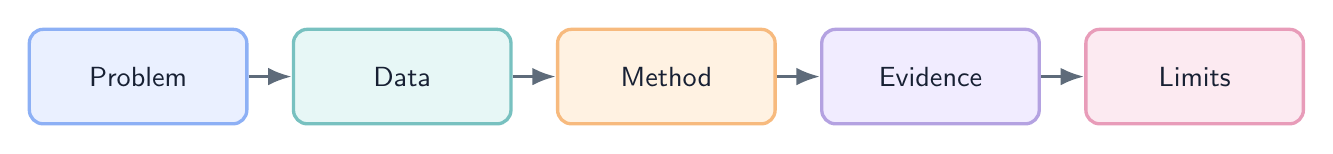
\begin{tikzpicture}[node distance=5.5mm]
\node[flowblue,text width=2.2cm] (p) {Problem};
\node[flowteal,text width=2.2cm,right=of p] (data) {Data};
\node[floworange,text width=2.2cm,right=of data] (method) {Method};
\node[flowpurple,text width=2.2cm,right=of method] (evi) {Evidence};
\node[flowpink,text width=2.2cm,right=of evi] (lim) {Limits};
\draw[arrow] (p)--(data);\draw[arrow] (data)--(method);\draw[arrow] (method)--(evi);\draw[arrow] (evi)--(lim);
\end{tikzpicture}
\end{center}

\begin{enumerate}
  \item 先展示一個具體使用情境，而不是先講模型架構。
  \item 明確定義輸入、輸出與成功條件。
  \item 架構圖說明資料如何流動。
  \item 用表格與曲線回答「是否比 baseline 好」。
  \item Demo 顯示代表性情況，不取代正式評估。
  \item 主動展示失敗案例與下一個最值得做的實驗。
\end{enumerate}


% ================================================================
% APPENDICES
% ================================================================
\appendix
\titleformat{\chapter}[display]
  {\bfseries\color{Ink}}
  {
\begin{tikzpicture}[baseline=(n.base)]\node[fill=Purple,text=white,rounded corners=4pt,inner xsep=9pt,inner ysep=4pt,font=\large\bfseries] (n) {APPENDIX \thechapter};\end{tikzpicture}}
  {8pt}{\Huge}[\vspace{3pt}\color{Line}\titlerule]

\chapter{術語速查表}

\begin{longtable}{>{\bfseries}p{3.6cm} p{4.1cm} p{8cm}}
\toprule
英文術語 & 中文角色 & 直觀解釋 \\
\midrule
\endfirsthead
\toprule
英文術語 & 中文角色 & 直觀解釋 \\
\midrule
\endhead
Pixel & 像素 & 影像中最小的顏色格子；模型最初看到的是像素數值。\\
Frame & 影格 & 影片中的一張靜態影像。\\
FPS & 每秒影格數 & 決定時間解析度；30 FPS 表示每秒 30 張。\\
BBOX & 邊界框 & 用矩形近似物件位置。\\
Keypoint & 關鍵點 & 有明確語意的點，例如手腕、球場線交點。\\
Segmentation mask & 分割遮罩 & 指出物件每個像素的精細區域。\\
Confidence & 信心分數 & 模型內部的排序分數，不一定是校準後正確率。\\
IoU & 交並比 & 兩個框重疊面積除以聯集面積。\\
NMS & 非極大值抑制 & 移除同一物件附近的重複候選框。\\
Homography & 平面單應性 & 將一個平面的座標映射到另一個平面。\\
BEV & 鳥瞰圖 & 將場地轉為接近俯視的共同座標。\\
Footpoint & 腳底接觸點 & 用來代表球員落在地板上的位置。\\
Tracking & 追蹤 & 跨影格維持同一物件的身分。\\
Track ID & 軌跡識別碼 & 影片內暫時身分，不等於球員姓名或背號。\\
Data association & 資料關聯 & 決定哪個 detection 應接到哪個 track。\\
Kalman Filter & 卡爾曼濾波 & 用動態模型預測狀態，再用觀測修正。\\
Hungarian algorithm & 匈牙利指派 & 在一對一限制下尋找最小總成本配對。\\
ReID & 再識別 & 用外觀 embedding 協助遮擋後重新連接身分。\\
Embedding & 特徵向量 & 將影像 crop 轉成可比較距離的向量。\\
Clustering & 分群 & 沒有標籤時，依特徵相似度自動分組。\\
Pose estimation & 姿態估計 & 預測人體關節位置。\\
Reprojection error & 重投影誤差 & 模型投影位置與已知真值位置的距離。\\
Baseline & 基準方法 & 合理的簡單比較對象。\\
Ablation & 消融實驗 & 拿掉某個模組，確認改進來源。\\
Domain shift & 領域偏移 & 訓練與實際環境的場館、光線、鏡頭或球衣不同。\\
\bottomrule
\end{longtable}

\chapter{工具選擇矩陣}

\begin{tabularx}{\textwidth}{>{\bfseries}p{3cm} Y Y Y}
\toprule
需求 & 優先考慮 & 優點 & 注意事項 \\
\midrule
快速建立 BBOX dataset & Roboflow / CVAT & UI 完整、協作與格式轉換方便 & 先寫標註規則，再開始大量標。\\
研究多種 detector & MMDetection & 配置與模型庫豐富 & 設定複雜，部署需額外整理。\\
快速完成 YOLO baseline & Ultralytics & 訓練、推論、track API 一致 & 版本更新快，需固定環境與參數。\\
幾何與相機處理 & OpenCV & 成熟、跨語言、函式完整 & 函式成功不代表點選擇正確。\\
靜態相機即時 MOT & ByteTrack & 簡潔、低額外成本 & 無 appearance，長遮擋易換 ID。\\
移動相機或較多 ID swap & BoT-SORT & 相機運動補償，可加 ReID & 參數與成本較高。\\
單人近距離即時 pose & MediaPipe & 輕量、容易整合 & 不等同高精度多人比賽 pose。\\
多人 pose 研究 & MMPose / OpenPose 系列 & 模型選擇與研究彈性高 & 遠距、小人物與遮擋仍具挑戰。\\
實驗追蹤 & W\&B / MLflow & 保存參數、曲線與 artifacts & 需先定義一致命名與資料版本。\\
\bottomrule
\end{tabularx}

\chapter{指標選擇速查}

\begin{tabularx}{\textwidth}{>{\bfseries}p{3.3cm} Y Y}
\toprule
任務 & 建議指標 & 同時要看的失敗案例 \\
\midrule
Detection & Precision、Recall、AP / mAP、small-object recall & 遠距球、重疊球員、裁判誤報。\\
Tracking & IDF1、HOTA、ID switches、coverage & 遮擋、交叉、攝影機運動。\\
Homography & validation reprojection error、court error & 視野邊緣、外插區域、相機位移。\\
Team classification & accuracy、macro F1、switch rate、reject rate & 白色球衣、陰影、裁判、背面。\\
Pose & PCK、OKS、Keypoint AP、角度誤差 & 遮擋、出畫、身體旋轉。\\
Event timing & frame MAE、tolerance accuracy & 出手型態不同、球短暫遺失。\\
End-to-end & 任務成功率、最終分析誤差、使用者時間 & 上游錯誤如何傳到結論。\\
\bottomrule
\end{tabularx}

\chapter{可延伸的專題方向}

\begin{enumerate}
  \item \textbf{球員位置分析：}比較 BBOX footpoint、腳踝 keypoint 與 segmentation footpoint 的 BEV 誤差。
  \item \textbf{追蹤穩定度：}比較 SORT、ByteTrack 與 BoT-SORT 在固定與移動相機下的 IDF1。
  \item \textbf{隊伍辨識：}比較 HSV、深度 embedding 與 track-level voting。
  \item \textbf{球權估計：}以球與球員距離、遮擋與時序狀態推論 possession。
  \item \textbf{投籃事件：}結合球軌跡、手腕距離與姿態訊號估計 release frame。
  \item \textbf{空間分析：}以 BEV 路徑計算 spacing、paint occupancy 與 transition speed。
  \item \textbf{姿態穩定：}比較單幀 Pose、移動平均與信心加權時序濾波對關節抖動與角度誤差的影響。
  \item \textbf{不確定性：}讓系統輸出位置區間、事件置信度與自動拒答，而非強制給單一答案。
\end{enumerate}

\renewcommand{\bibname}{參考資料與進一步閱讀}
\addcontentsline{toc}{chapter}{參考資料與進一步閱讀}
\small
\begin{thebibliography}{99}
\bibitem{ransac} Martin A. Fischler and Robert C. Bolles. Random Sample Consensus: A Paradigm for Model Fitting with Applications to Image Analysis and Automated Cartography. \textit{Communications of the ACM}, 1981.
\bibitem{hog} Navneet Dalal and Bill Triggs. Histograms of Oriented Gradients for Human Detection. CVPR, 2005.
\bibitem{rcnn} Ross Girshick et al. Rich Feature Hierarchies for Accurate Object Detection and Semantic Segmentation. CVPR, 2014.
\bibitem{fasterrcnn} Shaoqing Ren et al. Faster R-CNN: Towards Real-Time Object Detection with Region Proposal Networks. NeurIPS, 2015.
\bibitem{yolo} Joseph Redmon et al. You Only Look Once: Unified, Real-Time Object Detection. CVPR, 2016.
\bibitem{detr} Nicolas Carion et al. End-to-End Object Detection with Transformers. ECCV, 2020.
\bibitem{sort} Alex Bewley et al. Simple Online and Realtime Tracking. ICIP, 2016.
\bibitem{deepsort} Nicolai Wojke, Alex Bewley, and Dietrich Paulus. Simple Online and Realtime Tracking with a Deep Association Metric. ICIP, 2017.
\bibitem{bytetrack} Yifu Zhang et al. ByteTrack: Multi-Object Tracking by Associating Every Detection Box. ECCV, 2022.
\bibitem{botsort} Nir Aharon, Roy Orfaig, and Ben-Zion Bobrovsky. BoT-SORT: Robust Associations Multi-Pedestrian Tracking. arXiv:2206.14651, 2022.
\bibitem{hota} Jonathon Luiten et al. HOTA: A Higher Order Metric for Evaluating Multi-Object Tracking. International Journal of Computer Vision, 2021.
\bibitem{openpose} Zhe Cao et al. OpenPose: Realtime Multi-Person 2D Pose Estimation Using Part Affinity Fields. IEEE TPAMI, 2021.
\bibitem{hrnet} Ke Sun et al. Deep High-Resolution Representation Learning for Human Pose Estimation. CVPR, 2019.
\bibitem{blazepose} Valentin Bazarevsky et al. BlazePose: On-device Real-time Body Pose Tracking. arXiv:2006.10204, 2020.
\bibitem{integralpose} Xiao Sun et al. Integral Human Pose Regression. ECCV, 2018.
\bibitem{simcc} Yanjie Li et al. SimCC: a Simple Coordinate Classification Perspective for Human Pose Estimation. ECCV, 2022.
\bibitem{vitpose} Yufei Xu et al. ViTPose: Simple Vision Transformer Baselines for Human Pose Estimation. NeurIPS, 2022.
\bibitem{rtmpose} Tao Jiang et al. RTMPose: Real-Time Multi-Person Pose Estimation Based on MMPose. arXiv:2303.07399, 2023.
\bibitem{opencv} OpenCV Documentation. Basic Concepts of the Homography Explained with Code. \url{https://docs.opencv.org/4.x/d9/dab/tutorial_homography.html}
\bibitem{ultralytics} Ultralytics Documentation. Multi-Object Tracking with BoT-SORT and ByteTrack. \url{https://docs.ultralytics.com/modes/track/}
\bibitem{roboflow} Roboflow Documentation. Annotation Tools and Project Types. \url{https://docs.roboflow.com/annotate/annotation-tools}
\end{thebibliography}
\normalsize

\begin{heroBox}
\textbf{最後提醒：}\quad
本講義旨在建立一套可持續擴充的分析框架：先定義問題與輸出，再選資料與方法；保留中間結果，逐層評估；最後用證據支持結論，並清楚說明不能做什麼。
\end{heroBox}

\end{document}
